% !TeX root = bagrut-all.tex

\selectlanguage{hebrew}

\chapter{טריגונומטריה}


\section{קיץ תשע"ח מועד ב}

\begin{center}
\selectlanguage{english}
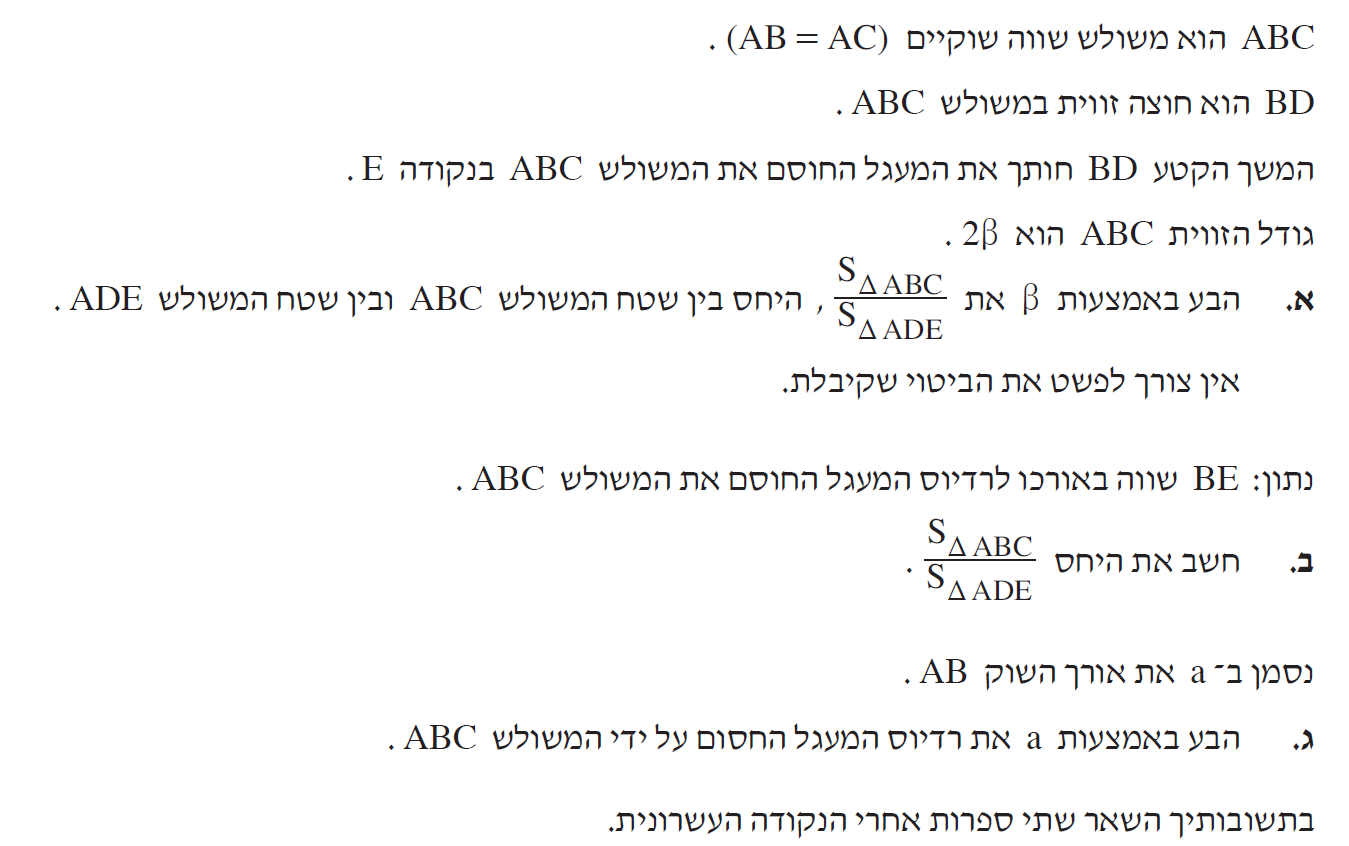
\includegraphics[width=\textwidth]{summer-2018b-5}
\end{center}

להלן תרשים עם הזוויות הנתונות ב-%
$B,C$,
ולאחר חישוב הזוויות האחרות לפי סכום של זוויות במשולש וזוויות משלימות.
$\angle EAC=\angle EBC=\beta$,
$\angle AEB=\angle ACB=2\beta$,
כי הן נשענות על אותן קשתות
$EC,AB$.
\begin{center}
\selectlanguage{english}
\begin{tikzpicture}[scale=1.4]
\clip(-5mm,-5mm) rectangle +(11,5.2);
\coordinate (B) at (0,0);
\coordinate (C) at (10,0);
\path[name path=ba] (B) -- +(40:7);
\path[name path=ca] (C) -- +(140:7);
\path[name intersections={of=ca and ba,by={A}}];
\draw[thick] (A) -- node[above] {$a$} (B) -- (C) -- cycle;
\path[name path=bd] (B) -- +(15:10);
\tkzCircumCenter(A,B,C)\tkzGetPoint{O}
\node[draw,very thick,dotted,circle through=(A),name path=circle] (circle) at (O) {};
\path[name intersections={of=bd and ca,by={D}}];
\path[name intersections={of=bd and circle,by={E}}];
\fill (A) node[above] {$A$} circle(1.5pt) node[below right,xshift=42pt,yshift=-22pt] {$\beta$} node[below,yshift=-20pt] {$180\!-\!4\beta$};
\fill (B) node[left,xshift=-4pt] {$B$} node[above right,xshift=50pt,yshift=-2pt] {$\beta$} node[above right,xshift=50pt,yshift=20pt] {$\beta$} circle(1.5pt);
\fill (C) node[right,xshift=4pt] {$C$} node[above left,xshift=-20pt,yshift=-1pt] {$2\beta$} circle(1.5pt);
\fill (D) node[above,yshift=2pt] {$D$} node[left,xshift=-15pt,yshift=3pt] {$3\beta$} node[below,xshift=-8,yshift=-12pt] {$180\!-\!3\beta$} circle(1.5pt);
\fill (E) node[above,right] {$E$} circle(1.5pt) node[left,xshift=-14pt] {$2\beta$};
\draw[thick] (B) -- (D) -- (E) -- (A);
\end{tikzpicture}
\end{center}

\np

\textbf{סעיף א}


$\triangle ABC$
משולש שוקיים ולפי הנוסחה הטריגונומטרית לשטח של משולש:
\[
S_{\triangle ABC}=\frac{1}{2}\cdot a\cdot a \cdot \sin (180\!-\!4\beta)=\frac{a^2}{2}\sin 4\beta\,.
\]
כדי שהיחס יהיה ביטוי ב-%
$\beta$
בלבד, עלינו למצוא ביטוי ל-%
$S_{\triangle ADE}$
כך ש-%
$a^2$
יצטמצם.

ב-%
$\triangle ABD$
ו-%
$\triangle ABE$
צלע אחת שווה
$a$
וצלע שנייה היא באורך
$AD$
ו-%
$AE$.
לפי חוק הסינוסים:
\erh{14pt}
\begin{equationarray*}{rcl}
\frac{AE}{\sin \beta}&=&\frac{a}{\sin 2\beta}\\
AE&=&\frac{a\sin\beta}{\sin 2\beta}\\
\frac{AD}{\sin \beta}&=&\frac{a}{\sin 3\beta}\\
AD&=&\frac{a\sin\beta}{\sin 3\beta}\\
S_{\triangle ADE}&=&\frac{1}{2}\cdot \frac{a\sin \beta}{\sin 2\beta}\cdot\frac{a\sin\beta}{\sin 3\beta}\cdot \sin \beta\\
&=&\frac{a^2}{2}\cdot \frac{\sin^3 \beta}{\sin 2\beta\sin 3\beta}\\
\frac{S_{\triangle ABC}}{S_{\triangle ADE}}&=&\frac{\sin 4\beta\sin 2\beta\sin 3\beta}{\sin^3\beta}\,.
\end{equationarray*}

הוכחה אחרת: לחשב
$AE$
או
$AD$,
ולהשתמש בחוק הסינוסים על
$\triangle ADE$
כדי לחשב את השני.


\textbf{סעיף ב}

נשתמש בחוק הסינוסים על 
$\triangle ABE$
עם צלע 
$BE$,
ומ-%
$R=BE$
הרדיוס יצטמצם:
\erh{12pt}
\begin{equationarray*}{rcl}
2R&=&\frac{BE}{\sin(180\!-\!4\beta+\beta)}=\frac{BE}{\sin 3\beta}=\frac{R}{\sin 3\beta}\\
2\sin 3\beta&=&1\\
3\beta&=&30^\circ\\
\beta&=&10^\circ\,.
\end{equationarray*}
נכון שגם
$\sin 3\cdot 50 = \frac{1}{2}$,
אבל לא ייתכן שלמשולש שתי זוויות של 
$2\cdot 50=100$.

עם ערכו של 
$\beta$
נוכל לחשב את יחס השטחים:
\[
\frac{S_{\triangle ABC}}{S_{\triangle ADE}}=\frac{\sin 4\beta\sin 2\beta\sin 3\beta}{\sin^3\beta}=\frac{\sin 40\sin 20\sin 30}{\sin^3 10}=20.99^\circ\,.
\]

\np

\textbf{סעיף ג}

לפי משפט
$6$
"במשולש שווה-שוקיים , חוצה זווית הראש, התיכון לבסיס והגובה לבסיס מתלכדים", כך שחוצה הזווית 
$\angle BAC$
ניצב ל-%
$BC$
בנקודה
$F$.
לפי משפט
$49$
"שלושת חוצי הזוויות של משולש נחתכים בנקודה אחת, שהיא מרכז המעגל החסום במשולש", הנקודה המסומנת 
$M$
בתרשים היא מרכז המעגל החסום.

\begin{center}
\selectlanguage{english}
\begin{tikzpicture}[scale=1.3]
\coordinate (B) at (0,0);
\coordinate (C) at (10,0);
\path[name path=ba] (B) -- +(20:6);
\path[name path=ca] (C) -- +(160:6);
\path[name intersections={of=ca and ba,by={A}}];
\draw[thick] (A) -- node[above,xshift=24pt,yshift=10pt] {$a$} (B) -- (C) -- cycle;
\path[name path=bd] (B) -- +(10:8.5);
\path[name intersections={of=bd and ca,by={D}}];
\fill (A) node[above] {$A$} circle(1.5pt);
\fill (B) node[left,xshift=-4pt] {$B$} node[above right,xshift=85pt,yshift=-1pt] {$\beta$} node[above right,xshift=85pt,yshift=16pt] {$\beta$} circle(1.5pt);
\fill (C) node[right,xshift=4pt] {$C$} circle(1.5pt);
\draw[thick] (B) -- (D);
\node at ($(A)+(-28pt,6pt)$) {$90\!-\!2\beta$};
\draw[->,thick] ($(A)+(-27pt,1pt)$) -- +(20pt,-10pt);
\coordinate (F) at ($(B)!(A)!(C)$);
\draw[rotate=90] (F) rectangle +(7pt,7pt);
\draw[thick,dashed,name path=altitude] (A) -- (F);
\path[name intersections={of=bd and altitude,by={M}}];
\fill (F) node[below] {$F$} circle(1.5pt);
\fill (M) node[above right] {$M$} circle(1.5pt);
\path (B) -- node[below] {$b$} (F);
\path (M) -- node[right] {$r$} (F);
\node[draw,very thick,dotted,circle through=(F),name path=circle] (circle) at (M) {};
\end{tikzpicture}
\end{center}
נשאר רק להשתמש בהגדרות של הפונקציות הטריגונומטריות. ב-%
$\triangle ABF$:
\erh{10pt}
\begin{equationarray*}{rcl}
\sin(90\!-\!2\beta)&=&\frac{b}{a}\\
b&=&a\cos 2\beta\,.
\end{equationarray*}

\vspace{-4ex}
ב-%
$\triangle BMF$:
\vspace{-4ex}
\erh{10pt}
\begin{equationarray*}{rcl}
\tan\beta&=&\frac{r}{b}\\
r&=&a\cos 2\beta\tan\beta\\
&=&a\cos 20\tan 10=0.1657a\,.
\end{equationarray*}

%%%%%%%%%%%%%%%%%%%%%%%%%%%%%%%%%%%%%%%%%%%%%%%%%%%%%%%%%%%%%%

\np

\section{קיץ תשע"ח מועד א}

\begin{center}
\selectlanguage{english}
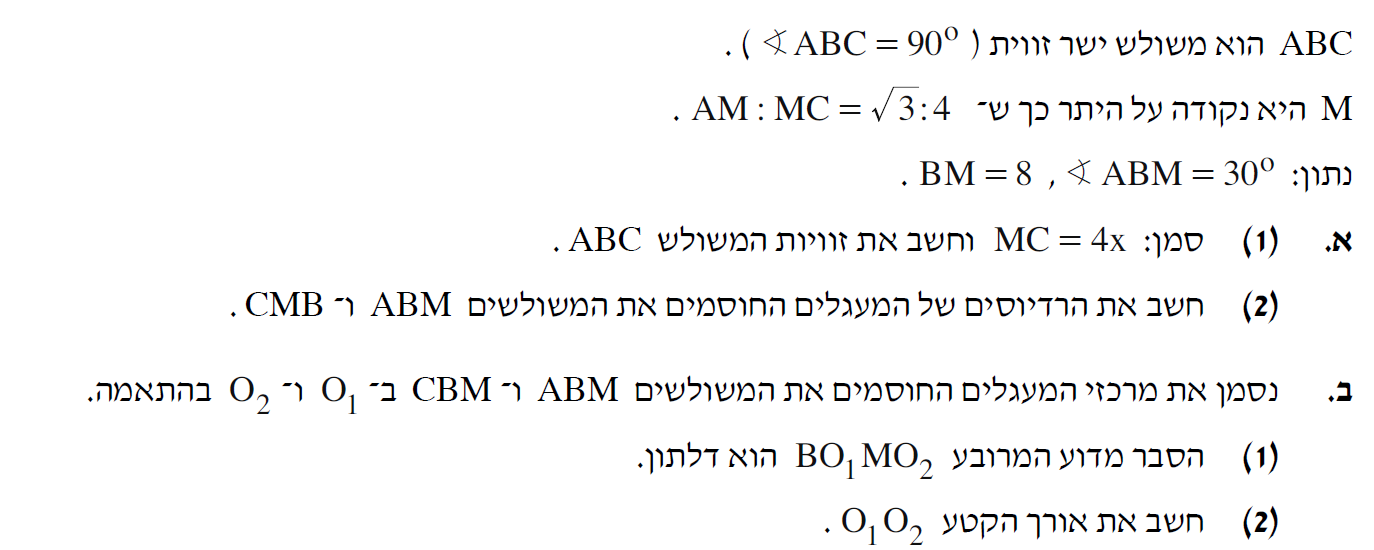
\includegraphics[width=\textwidth]{summer-2018a-5}
\end{center}

\vspace{-4ex}

\begin{center}
\selectlanguage{english}
\begin{tikzpicture}[scale=.9]
\coordinate (C) at (0,0);
\coordinate (B) at (7,0);
\path[name path=ca] (C) -- +(36:9);
\path[name path=ba] (B) -- +(90:5.5);
\path[name intersections={of=ca and ba,by={A}}];
\draw[thick] (A) -- (B) -- (C) -- cycle;
\coordinate (M) at ($(C)!{4/(sqrt(3)+4)}!(A)$);
\fill (C) node[left] {$C$} node[above right,xshift=18pt] {$90\!-\!\alpha$}circle(1.5pt);
\fill (B) node[right] {$B$} node[above left,xshift=-10pt] {$60$} node[above left,xshift=2pt,yshift=24pt] {$30$} circle(1.5pt);
\fill (A) node[right] {$A$} node[below left,xshift=2pt,yshift=-8pt] {$\alpha$} circle(1.5pt);
\fill (M) node[above left] {$M$} circle(1.5pt);
\draw[thick] (B) -- node[left,xshift=-3pt] {$8$} (M);
\path (C) -- node[above,xshift=-4pt] {$4x$} (M) -- node[above,xshift=-6pt] {$\sqrt{3}x$} (A);
\draw[rotate=90] (B) rectangle +(8pt,8pt);
\end{tikzpicture}
\end{center}

\vspace{-2ex}

\textbf{סעיף א}

$(1)$
נסמן
$\angle BAM=\alpha, \angle BCM=90\!-\!\alpha$.
לשני המשולשים 
$\triangle ABM,\triangle CMB$
צלע עם הנעלם
$x$,
זווית ידועה אחת, וזווית שנייה עם הנעלם 
$\alpha$.
מחוק הסינוסים נקבל שתי משוואות עם שני הנעלמים שאפשר לפתור כדי לקבל משוואה אחת עם הנעלם
$\alpha$
בלבד:
\erh{14pt}
\begin{equationarray*}{rcl}
\frac{\sqrt{3}x}{\sin 30}&=&\frac{8}{\sin\alpha}\\
x&=&\frac{8\sin 30}{\sqrt{3}\sin\alpha}=\frac{4}{\sqrt{3}\sin \alpha}\\
\frac{4x}{\sin 60}&=&\frac{8}{\sin (90\!-\!\alpha)}\\
x&=&\frac{8\sin 60}{4\cos\alpha}=\frac{\sqrt{3}}{\cos\alpha}\\
\tan \alpha&=&\frac{4}{\sqrt{3}\sqrt{3}}=\frac{4}{3}\,.
\end{equationarray*}
חישוב עם מחשבון נותן
$\angle BAC=\alpha \approx 53.13$,
ולא נשכח לרשום גם 
$\angle BCA=90\!-\!\alpha\approx 36.87$.

\np

$(2)$
נחשב 
$\sin 53.13\approx 0.8, \cos 53.13\approx 0.6$.
אפשר לקבל ערכים רציונליים על ידי שימוש בנוסחאות )שאינן נמצאות בנוסחאון(:
\erh{12pt}
\begin{equationarray*}{rcl}
\sin \alpha &=& \frac{\tan \alpha}{\sqrt{1+\tan^2\alpha}}=\frac{4/3}{\sqrt{1+(4/3)^2}}=\frac{4}{5}\\
\cos \alpha &=& \frac{1}{\sqrt{1+\tan^2\alpha}}=\frac{1}{\sqrt{1+(4/3)^2}}=\frac{3}{5}\,.
\end{equationarray*}
נשתמש בחוק הסינוסים עבור 
$\triangle ABM$, $\triangle CMB$:
\erh{12pt}
\[
\begin{array}{rcl@{\hspace{3em}}rcl}
2R_1&=&\disfrac{8}{\sin\alpha},&R_1&=&4\cdot \disfrac{5}{4}=5\\
2R_2&=&\disfrac{8}{\sin(90\!-\!\alpha)},&R_2&=&4\cdot \disfrac{5}{3}=20/3\,.
\end{array}
\]

\vspace{-1ex}

\textbf{סעיף ב}

$(1)$
$O_1M=O_1B$
כי הם רדיוסים של המעגל החוסם את
$\triangle ABM$,
ו-%
$O_2M=O_2B$
כי הם רדיוסים של המעגל החוסם את
$\triangle CBM$.
לפי ההגדרה מרובע עם שני זוגות של צלעות שכנות שהן שוות הוא דלתון.
\begin{center}
\selectlanguage{english}
\begin{tikzpicture}[scale=1.1]
\clip (-6mm,-5mm) rectangle +(11,6);
\coordinate (C) at (0,0);
\coordinate (B) at (7,0);
\path[name path=ca] (C) -- +(36:9);
\path[name path=ba] (B) -- +(90:5.5);
\path[name intersections={of=ca and ba,by={A}}];
\draw[thick] (A) -- (B) -- (C) -- cycle;
\coordinate (M) at ($(C)!{4/(sqrt(3)+4)}!(A)$);
\fill (C) node[left] {$C$} circle(1.5pt);
\fill (B) node[right] {$B$} circle(1.5pt);
\fill (A) node[right] {$A$} circle(1.5pt);
\fill (M) node[above left] {$M$} circle(1.5pt);
\draw[thick] (B) -- (M);
\tkzCircumCenter(A,B,M)\tkzGetPoint{O1}
\tkzCircumCenter(C,B,M)\tkzGetPoint{O2}
\fill (O1) node[above right] {$O_1$} circle(1.5pt);
\fill (O2) node[above left] {$O_2$} circle(1.5pt);
\node [draw,thick,dotted,circle through=(M)] (circle) at (O1) {};
\node [draw,thick,dotted,circle through=(M)] (circle) at (O2) {};
\draw[thick] (O1) -- node[right] {$R_1$} (B) -- node[below,yshift=-3pt] {$R_2$} (O2) -- node[left] {$R_2$} (M) -- node[above] {$R_1$} cycle;
\draw[thick,name path=diagonal1] (O1) -- (O2);
\path[name path=diagonal2] (M) -- (B);
\path[name intersections={of=diagonal1 and diagonal2,by={E}}];
\fill (E) node[left,xshift=-3pt,yshift=2pt] {$E$} circle(1.5pt);
\draw[rotate=32] (E) rectangle +(7pt,7pt);
\path (M) -- node[left] {$4$} (E) -- node[left,xshift=-3pt,yshift=4pt] {$4$} (B);
\end{tikzpicture}
\end{center}

$(2)$
לפי משפט
$21$
"האלכסון הראשי בדלתון חוצה את זוויות הראש, חוצה את האלכסון השני ומאונך לו".
מכאן
$\angle MEO_1=\angle MEO_2=90$.
נתון
$MB=8$
ולכן
$ME=EB=4$.
לפי משפט פיתגורס:

\vspace{-6ex}

\erh{18pt}
\begin{equationarray*}{rcl}
O_1O_2=O_1E+O_2E&=&\sqrt{R_1^2-16} + \sqrt{R_2^2-16}\\
&=&\sqrt{5^2-16} + \sqrt{\left(\frac{20}{3}\right)^2-16}=3+\frac{16}{3}=\frac{25}{3}\,.
\end{equationarray*}

%%%%%%%%%%%%%%%%%%%%%%%%%%%%%%%%%%%%%%%%%%%%%%%%%%%%%%%%%%%%%%

\np


\section{חורף תשע"ח}

\begin{center}
\selectlanguage{english}
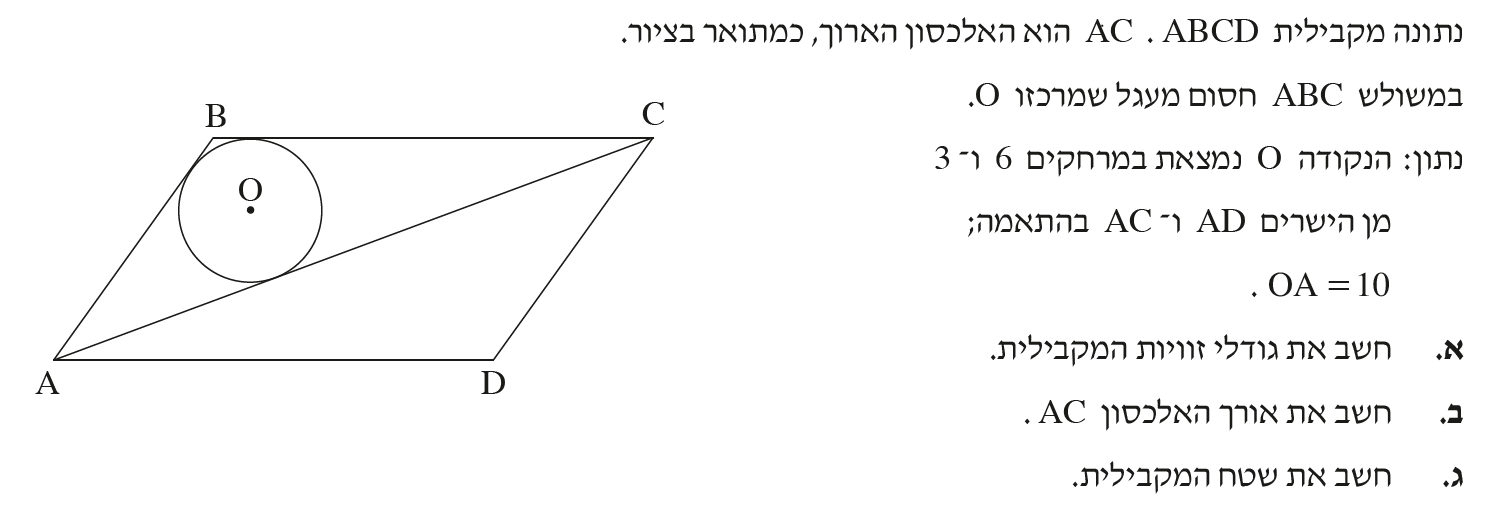
\includegraphics[width=\textwidth]{winter-2018-5}
\end{center}

\vspace{-1ex}

$E,F$
הן נקודות המפגש של האנכים מ-%
$O$
עם 
$AC,AD$.
לפי משפט
$49$
"שלושת חוצי הזוויות של משולש נחתכים בנקודה אחת, שהיא מרכז המעגל החסום במשולש", 
$AO,CO$
הם חוצי הזוויות
$BAC,BCA$,
בהתאמה. ניסיתי לפתור את השאלה תוך הנחה שאלכסון של מקבילית חוצה את הזוויות
$\angle BAC=\angle BCD$.
כמובן שזה נכון רק עבור מעוין.

במשולשים ישר-זווית
$\triangle AOE, \triangle AOF$
נסמן את הזוויות
$\alpha=\angle OAE,\beta=\angle OAF$.

\vspace{-2ex}

\begin{center}
\selectlanguage{english}
\begin{tikzpicture}%[scale=1.1]
\clip (-12mm,-5.5mm) rectangle +(12.5,5);
\coordinate (A) at (0,0);
\coordinate (D) at (8,0);
\coordinate (B) at (54:4.5);
\coordinate (C) at ($(D)+(54:4.5)$);
\fill (A) node[below] {$A$} circle(1.5pt);
\fill (B) node[above] {$B$} circle(1.5pt);
\fill (C) node[above] {$C$} circle(1.5pt);
\fill (D) node[below] {$D$} circle(1.5pt);
\draw[thick] (D) -- (A) -- (B) -- (C) -- cycle;
\draw[thick] (A) -- (C);
\tkzInCenter(A,B,C)\tkzGetPoint{O}
\fill (O) node[above] {$O$} circle(1.5pt);
\node[draw,thick,circle through=($(B)!(O)!(C)$),name path=circle] at (O) {};
\draw[thick,dashed] (A) -- node[left,near end,xshift=10pt,yshift=12pt] {$10$} (O) -- (C);
\coordinate (E) at ($(A)!(O)!(C)$);
\coordinate (F) at ($(A)!(O)!(D)$);
\fill (E) node[below right] {$E$} circle(1.5pt);
\fill (F) node[below] {$F$} circle(1.5pt);
\draw[thick,dashed] (E) -- node[right,near end] {$3$} (O) -- node[right,near end] {$6$} (F);
\draw[rotate=19] (E) rectangle +(7pt,7pt);
\draw (F) rectangle +(7pt,7pt);
\draw[thick] ($(A)+(20mm,0)$) arc[start angle=0,end angle=37,radius=20mm];
\node[right,xshift=54pt,yshift=12pt] at (A) {$\beta$};
\node[above right,xshift=34pt,yshift=14pt] at (A) {$\alpha$};
\node[above right,xshift=28pt,yshift=28pt] at (A) {$\alpha$};
\node at (-2mm,2.5) {$\angle OAF=\beta$};
\end{tikzpicture}
\end{center}

\vspace{-2ex}

\textbf{סעיף א}

לפי התרשים
$\angle BAD=\alpha+\beta$.
נחשב
$\alpha,\beta$
מהפונקציות הטריגונומטריות במשולשים ישר-זווית:
\erh{12pt}
\begin{equationarray*}{rcl}
\sin \alpha &=& 3/10,\quad\quad \alpha = 17.46\\
\sin \beta &=& 6/10,\quad\quad \beta = 36.87\\
\angle BCD =\angle BAD&=& \alpha+\beta=54.33\\
\angle ABC =\angle ADC&=& \frac{360-2(\alpha+\beta)}{2}=125.67\,.
\end{equationarray*}

\np


\textbf{סעיף ב}

האלכסון
$AC$
הוא צלע של
$\triangle ABC$
והזוויות שלו ידועים, אבל אי-אפשר להשתמש בחוק הסינוסים כי אורכי הצלעות לא ידועים. מהתרשים רואים שהאלכסון מורכב משני קטעי קו
$AE,EC$
שהם צלעות של משולשים ישר-זווית
$\triangle AOE, \triangle COE$.
$AE$
מתקבל ממשפט פיתגורס:
\[
AE = \sqrt{10^2-3^2}=9.54\,.
\]
נשתמש בחוק הסינוסים ב-%
$\triangle COE$
)ונימנע מהפיתוי לקבוע ש-%
$\angle OCE=\alpha$(.
לפי זוויות מתחלפות
$\angle BCA=\angle CAD=\beta-\alpha$.
נזכור ש-%
$CE$
חוצה זווית ונקבל:

\vspace{-2ex}

\erh{12pt}
\begin{equationarray*}{rcl}
\angle OCE=\frac{\angle BCA}{2}&=&\frac{\beta-\alpha}{2} =\frac{36.87-17.46}{2}=9.71\\
\angle COE &=& 180-90-\angle OCE=80.29\\
\frac{EC}{\sin 80.29}&=& \frac{3}{\sin 9.71}\\
EC&=&17.54\\
AC=AE+EC&=&9.54+17.54=27.08\,.
\end{equationarray*}

\vspace{-2ex}

\textbf{סעיף ג}

שטח של מקבילית הוא הבסיס כפול הגובה:

\begin{center}
\selectlanguage{english}
\begin{tikzpicture}[scale=.7]
\coordinate (A) at (0,0);
\coordinate (B) at (54:4.5);
\coordinate (D) at (8,0);
\coordinate (C) at ($(D)+(54:4.5)$);
\fill (A) node[below] {$A$} node[above right,xshift=46pt,yshift=0pt] {$\beta-\alpha$} node[above right,xshift=16pt,yshift=10pt] {$2\alpha$} circle(1.5pt);
\fill (B) node[above] {$B$} circle(1.5pt);
\fill (C) node[above] {$C$} circle(1.5pt);
\fill (D) node[below] {$D$} circle(1.5pt);
\draw[thick] (D) -- node[below] {$b$} (A) -- node[above,yshift=2pt] {$27.08$} (C) -- cycle;
\draw[thick] (A) -- (B) -- (C);
\coordinate (H) at ($(A)!(C)!(D)$);
\fill (H) node[below] {$H$} circle(1.5pt);
\draw[rotate=90] (H) rectangle +(10pt,10pt);
\draw[thick,dashed] (D) -- (H) -- node[right] {$h$} (C);
\node[above left,xshift=-2pt,yshift=2pt] at (D) {$125.67$};
\node[below left,xshift=-16pt,yshift=-12pt] at (C) {$2\alpha$};
\end{tikzpicture}
\end{center}

\vspace{-4ex}

\erh{12pt}
\begin{equationarray*}{rcl}
\frac{b}{\sin 2\alpha}=\frac{b}{\sin 34.92}&=&\frac{27.08}{\sin 125.67}\\
b&=&19.08\\
\sin (\beta-\alpha)=\sin 19.41 &=& \frac{h}{27.08}\\
h&=&9\\
S_{ABCD}=bh&=&171.71\,.
\end{equationarray*}

\vspace{-2ex}


אפשרות אחרת היא לחשב את 
$AB$
לפי חוק הסינוסים, 
$S_{\triangle ABC}=\frac{1}{2}AB\cdot AB\sin \angle BAC$,
ולהכפיל בשניים.

%%%%%%%%%%%%%%%%%%%%%%%%%%%%%%%%%%%%%%%%%%%%%%%%%%%%%%%%%%%%%%

\np

\section{קיץ תשע"ז מועד ב}

\begin{center}
\selectlanguage{english}
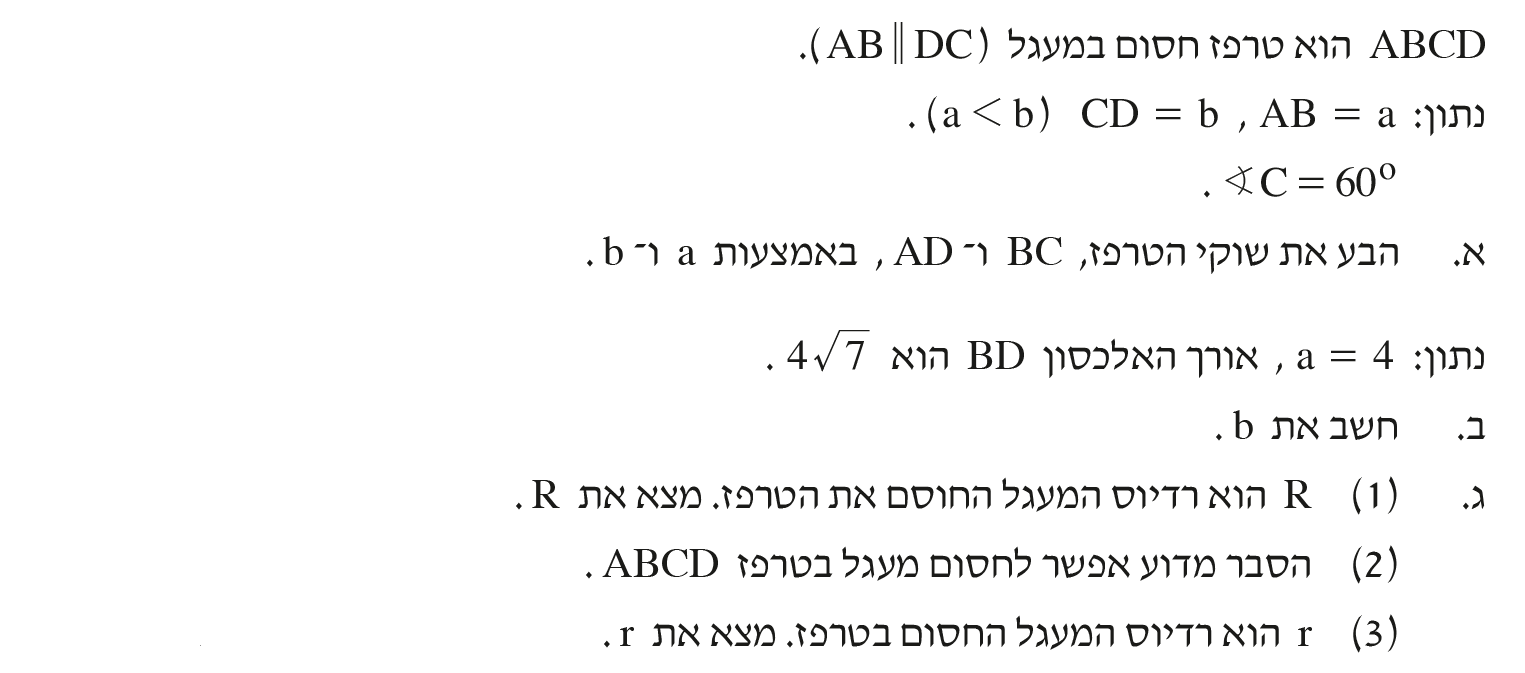
\includegraphics[width=\textwidth]{summer-2017b-5}
\end{center}

\vspace{-1ex}

\textbf{סעיף א}


לפי משפט
$56$
"ניתן לחסום מרובע במעגל אם ורק אם סכום זוג זוויות נגדיות שווה ל-%
$180$",
ולכן
$\angle DAB=120$.
נוריד גבהים מ-%
$A,B$
ל-%
$CD$
החותכים אותו ב-%
$E,F$.
$\triangle AED,\triangle BFC$
הם משולשים ישר-זווית. בתרשים השלמנו את הזוויות במשולשים ל-%
$180$.
לפי משפט
$40$
"טרפז בו הזוויות שליד אותו בסיס שוות זו לזו הוא טרפז שווה-שוקיים", ולכן
$ABCD$
שווה-שוקיים.
\begin{center}
\selectlanguage{english}
\begin{tikzpicture}[scale=1.1]
\clip (-.5,-.5) rectangle +(9,4.25);
\draw[thick] (0,0) coordinate (D) node[below left] {$D$} -- node[below] {$b$} (8,0) coordinate (C) node[below right] {$C$};
\fill (C) node[above left,xshift=-4pt] {$60$} circle(1.5pt);
\fill (D) node[above right,xshift=4pt] {$60$} circle(1.5pt);
\path[name path=s1] (D) -- +(60:4);
\path[name path=s2] (C) -- +(120:4);
\path[name path=top] (1,3) -- (7,3);
\path[name intersections={of=s1 and top,by={A}}];
\path[name intersections={of=s2 and top,by={B}}];
\fill (A) node[above left] {$A$} node[below right] {$90$} node[below,xshift=-8pt,yshift=-22pt] {$30$}  circle(1.5pt);
\fill (B) node[above right] {$B$} node[below left] {$90$}  node[below,xshift=8pt,yshift=-22pt] {$30$} circle(1.5pt);
\draw[thick] (D) -- node[left] {$s$} (A) -- node[above] {$a$} (B) -- node[right] {$s$} (C);
\tkzCircumCenter(A,B,C)\tkzGetPoint{O}
\tkzDrawCircle[thick,dotted,name path=circle](O,A)
\coordinate (E) at (D-|A);
\fill (E) node[below] {$E$} circle(1.5pt);
\draw[thick,dashed] (A) -- (E);
\draw (E) rectangle +(7pt,7pt);
\coordinate (F) at (D-|B);
\fill (F) node[below] {$F$} circle(1.5pt);
\draw[thick,dashed] (B) -- (F);
\draw[rotate=90] (F) rectangle +(7pt,7pt);
\draw[dashed] (A) -- node[below,xshift=-4pt] {$c$} (C);
\end{tikzpicture}
\end{center}
$AE=BF$
כך ש-%
$\triangle AED\cong\triangle BFC$.
מכאן:

\vspace{-2ex}

\erh{6pt}
\begin{equationarray*}{rcl}
\cos 60 &=& \frac{(b-a)/2}{s}=\frac{1}{2}\\
s&=&b-a\,.
\end{equationarray*}

\vspace{-4ex}

פתרון אחר משתמש בחוק הקוסינוסים על 
$\triangle ACD,\triangle ACB$.
נסמן ב-%
$c$
את אורך האלכסון
$AC$.

\vspace{-2ex}

\erh{2pt}
\begin{equationarray*}{rcl}
c^2 &=& s^2+b^2-2sb\cos 60\\
&=& s^2-sb+b^2\\
c^2 &=& s^2+a^2-2sa\cos 120\\
&=& s^2+sa+a^2
\end{equationarray*}
\vspace{-3ex}

נשווה את שתי הנוסחאות ל-%
$c^2$,
והפתרון הוא
$s=b-a$.

\np

\textbf{סעיף ב}

שקלתי להשתמש בחוק הסינוסים במשלוש
$\triangle ADB$:
פעם אחת לחשב 
$\angle ADB$
ופעם שנייה לחשב את
$s$.
עדיף להשתמש בחוק הקוסינוסים ב-%
$\triangle ADB$
כי אנו יודעים ש-%
$s=b-a=b-4$:
\erh{3pt}
\begin{equationarray*}{rcl}
(4\sqrt{7})^2&=&4^2+(b-4)^2-2\cdot 4\cdot (b-4)\cdot \cos 120\\
b^2-4b-96&=&(b-12)(b+8)=0\\
b&=&12\,.
\end{equationarray*}

\vspace{-2ex}

\begin{center}
\selectlanguage{english}
\begin{tikzpicture}[scale=1.1]
\clip (-.5,-.5) rectangle +(9,4.25);
\draw[thick] (0,0) coordinate (D) node[below left] {$D$} -- node[above] {$b$} (8,0) coordinate (C) node[below right] {$C$};
\fill (C) node[above left,xshift=-4pt] {$60$} circle(1.5pt);
\fill (D) circle(1.5pt);
\path[name path=s1] (D) -- +(60:4);
\path[name path=s2] (C) -- +(120:4);
\path[name path=top] (1,3) -- (7,3);
\path[name intersections={of=s1 and top,by={A}}];
\path[name intersections={of=s2 and top,by={B}}];
\fill (A) node[above left] {$A$} node[below right] {$120$} circle(1.5pt);
\fill (B) node[above right] {$B$} circle(1.5pt);
\draw[thick] (D) -- node[left,xshift=-14pt] {$b-4$} (A) -- node[above] {$4$} (B) -- node[right,xshift=14pt] {$b-4$} (C);
\tkzCircumCenter(A,B,C)\tkzGetPoint{O}
\tkzDrawCircle[thick,dotted,name path=circle](O,A)
\fill (O) circle(3pt);
\coordinate (E) at (D-|A);
\coordinate (F) at (D-|B);
\fill (F) node[below] {$F$} circle(1.5pt);
\draw[thick,dashed] (B) -- node[left] {$2r$} (F);
\draw[rotate=90] (F) rectangle +(7pt,7pt);
\draw[thick,dashed] (B) -- node[below] {$4\sqrt{7}$} (D);
\end{tikzpicture}
\end{center}


\textbf{סעיף ג}

$(1)$
שימו לב שהאלכסון
$BD$
הוא 
\textbf{לא}
הקוטר של המעגל החוסם שמסומן בנקודה השחורה הגדולה. לפי חוק הסינוסים ב-%
$\triangle ADB$:
\[
R = \frac{4\sqrt{7}}{2\sin 120} = \frac{4\sqrt{7}}{\sqrt{3}}=6.11\,.
\]

\vspace{-1ex}

$(2)$
לפי משפט
$57$,
"מרובע קמור חוסם מעגל אם ורק אם סכום שתי צלעות נגדיות שווה לסכום שתי הצלעות הנגדיות האחרות":

\vspace{-4ex}

\erh{3pt}
\begin{equationarray*}{rcl}
a+b&\stackrel{?}{=}&s+s\\
a+b&\stackrel{?}{=}&(b-a)+(b-a)\\
3a&\stackrel{?}{=}&b\\
3\cdot 4&=&12\,.
\end{equationarray*}

\vspace{-4ex}

$(3)$
$AB,CD$
הם משיקים מקבילים למעגל החסום, ולכן
$BF=2r$:
\erh{14pt}
\begin{equationarray*}{rcl}
\sin 60 &=& \frac{2r}{s}=\frac{2r}{b-a}=\frac{2r}{8}\\
r&=&\frac{1}{2}\cdot\frac{\sqrt{3}}{2}\cdot 8 = 2\sqrt{3}=3.464\,.
\end{equationarray*}

%%%%%%%%%%%%%%%%%%%%%%%%%%%%%%%%%%%%%%%%%%%%%%%%%%%%%%%%%%%%%%


\np


\section{קיץ תשע"ז מועד א}

\begin{center}
\selectlanguage{english}
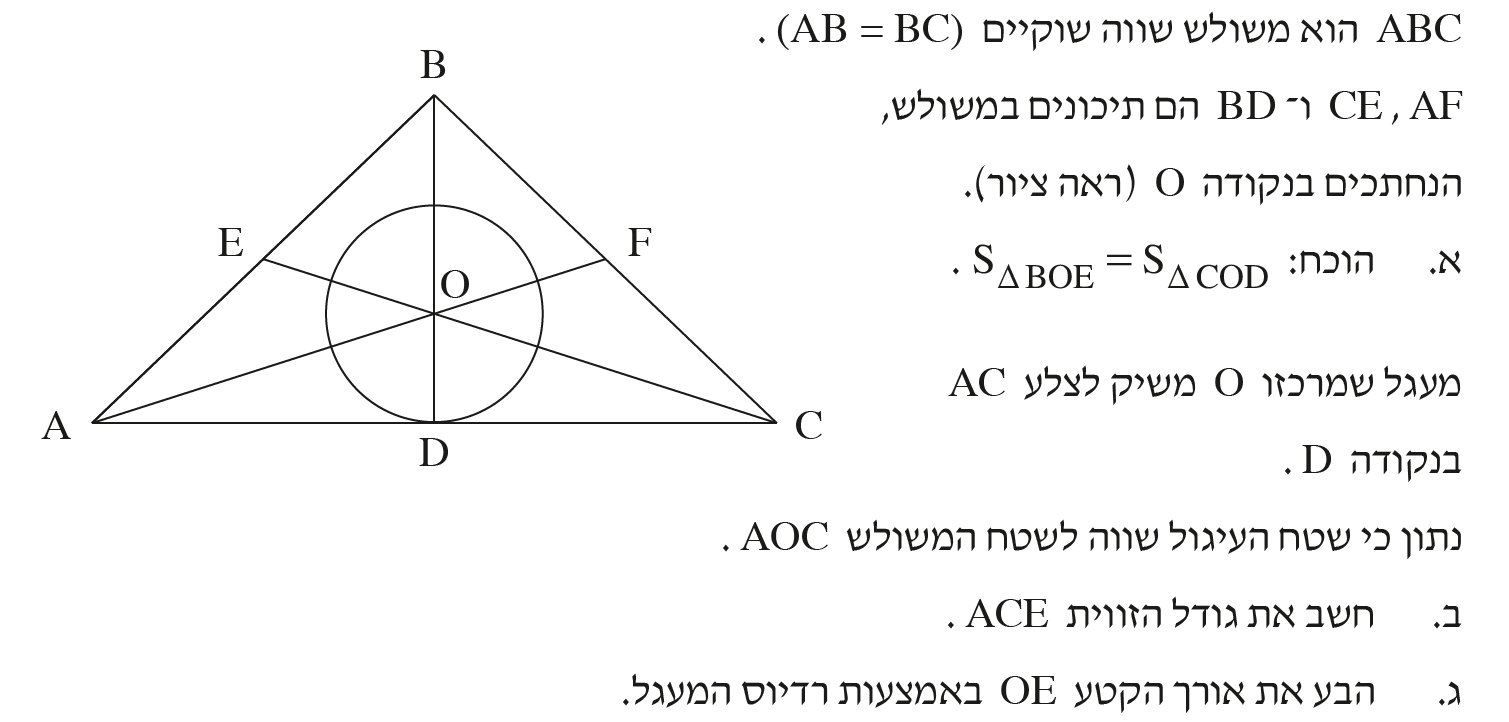
\includegraphics[width=\textwidth]{summer-2017a-5}
\end{center}

\vspace{-2ex}

\textbf{סעיף א}

נסמן אורכי צלעות בתרשים לפי
$\triangle ABC$
שווה-שוקיים,
$AF,BD,CF$
תיכונים, ומשפט
$46$
"נקודת חיתוך התיכונים מחלקת כל תיכון ביחס 
$2\!:\!1$".
כמו כן, 
$AF=CE$
כי
$\triangle CAF\cong \triangle ACE$
לפי צלע 
$AC=a$
משותף, זווית
$\angle CAE=\angle ACF$
)משולש שווה-שוקיים(, צלע
$AE=CF=b$.
\begin{center}
\selectlanguage{english}
\begin{tikzpicture}[scale=1.1]
\draw[thick] (0,0) coordinate (A) node[left] {$A$} -- (8,0) coordinate (C) node[right] {$C$} -- (4,4.5) coordinate (B) node[above] {$B$} -- cycle;
\fill (A) circle(1.5pt);
\fill (B) circle(1.5pt);
\fill (C) circle(1.5pt);
\coordinate (D) at ($(A)!.5!(C)$);
\coordinate (E) at ($(A)!.5!(B)$);
\coordinate (F) at ($(C)!.5!(B)$);
\fill (D) node[below] {$D$} circle(1.5pt);
\fill (E) node[left,xshift=-2pt,yshift=2pt]  {$E$} circle(1.5pt);
\fill (F) node[right,xshift=2pt,yshift=2pt] {$F$} circle(1.5pt);
\draw (D) rectangle +(8pt,8pt);
\draw[thick,name path=af] (A) -- (F);
\draw[thick,name path=ce] (C) -- (E);
\draw[thick,name path=bd] (B) -- (D);
\path[name intersections={of=af and ce,by={O}}];
\fill (O) node[above right,yshift=2pt] {$O$} node[above left,xshift=2pt,yshift=2pt] {$\alpha$} node[below right,xshift=-2pt,yshift=-2pt] {$\alpha$} circle(1.5pt);
\path (A) -- node[below] {$a/2$} (D) -- node[below] {$a/2$} (C);
\path (A) -- node[left] {$b/2$} (E) -- node[left] {$b/2$} (B);
\path (C) -- node[right] {$b/2$} (F) -- node[right] {$b/2$} (B);
\path (B) -- node[right] {$2r$} (O) -- node[right] {$r$} (D);
\path (A) -- node[above] {$2c$} (O) -- node[below] {$c$} (F);
\path (C) -- node[above] {$2c$} (O) -- node[below] {$c$} (E);
\draw[thick,dashed,name path=ef] (E) -- (F);
\path[name intersections={of=ef and bd,by={G}}];
\fill (G) node[above left] {$G$} circle(1.5pt);
\draw (G) rectangle +(7pt,7pt);
\end{tikzpicture}
\end{center}
$\triangle EBF\sim \triangle ABC$
לפי צ.ז.צ., ולכן
$EF=\frac{AC}{2}=\frac{a}{2}$.
$\triangle EBF$
גם הוא שווה-שוקיים, ולכן,
$BG$
הוא תיכון של
$EF$
ו-%
$EG=\frac{EF}{2}=\frac{a}{4}$.
\erh{16pt}
\begin{equationarray*}{rcl}
S_{\triangle BOE}&=&\frac{1}{2}\cdot EG\cdot BO=\frac{ar}{4}\\
S_{\triangle COD} &=& \frac{1}{2}\cdot OD\cdot DC =\frac{ar}{4}\,.
\end{equationarray*}

\np


פתרון אחר מתקבל מהנוסחה הטריגונומטרית לשטח עם הזוויות הקודקודיות 
$\alpha$:

\vspace{-4ex}

\erh{14pt}
\begin{equationarray*}{rcl}
S_{\triangle BOE}&=&\frac{1}{2}\cdot 2r\cdot c\cdot \sin \alpha\\
S_{\triangle COD}&=&\frac{1}{2}\cdot r\cdot 2c\cdot \sin \alpha\,.
\end{equationarray*}
\textbf{סעיף ב}

נסמן 
$\angle ACE=\beta$.
\begin{center}
\selectlanguage{english}
\begin{tikzpicture}[scale=1.1]
\draw[thick] (0,0) coordinate (A) node[left] {$A$} -- (8,0) coordinate (C) node[right] {$C$} -- (4,4.5) coordinate (B) node[above] {$B$} -- cycle;
\fill (A) circle(1.5pt);
\fill (B) circle(1.5pt);
\fill (C) node[left,xshift=-35pt,yshift=6pt] {$\beta$} circle(1.5pt);
\coordinate (D) at ($(A)!.5!(C)$);
\coordinate (E) at ($(A)!.5!(B)$);
\coordinate (F) at ($(C)!.5!(B)$);
\fill (D) node[below] {$D$} circle(1.5pt);
\fill (E) node[left,xshift=-2pt,yshift=2pt]  {$E$} circle(1.5pt);
\fill (F) node[right,xshift=2pt,yshift=2pt] {$F$} circle(1.5pt);
\draw (D) rectangle +(7pt,7pt);
\draw[thick,name path=af] (A) -- (F);
\draw[thick,name path=ce] (C) -- (E);
\draw[thick,name path=bd] (B) -- (D);
\path[name intersections={of=af and ce,by={O}}];
\fill (O) node[above right,yshift=2pt] {$O$} circle(1.5pt);
\path (A) -- node[below] {$a/2$} (D) -- node[below] {$a/2$} (C);
\path (B) -- node[right,near start] {$2r$} (O) -- node[right] {$r$} (D);
\path (A) -- node[above] {$2c$} (O) -- node[below] {$c$} (F);
\path (C) -- node[above] {$2c$} (O) -- node[below] {$c$} (E);
\node [draw,thick,circle through=(D),name path=circ] (circle) at (O) {};
\end{tikzpicture}
\end{center}

\vspace{-2ex}
נתון:
\vspace{-4ex}

\erh{12pt}
\begin{equationarray*}{rcl}
S_O&=&\pi r^2 = \frac{1}{2} ar = S_{\triangle AOC}\\
a &=& 2\pi r\,.
\end{equationarray*}

\vspace{-4ex}

נציב עבור 
$a$
בחישוב הטנגס של
$\beta$:
\erh{14pt}
\begin{equationarray*}{rcl}
\tan \beta &=& \frac{r}{a/2} = \frac{2r}{2\pi r}=\frac{1}{\pi}\\
\beta &=& \tan^{-1} \frac{1}{\pi}= 17.66^\circ\,.
\end{equationarray*}

\vspace{-2ex}

\textbf{סעיף ג}

נחשב סינוס של
$\beta$:

\vspace{-5ex}

\erh{14pt}
\begin{equationarray*}{rcl}
\sin \beta &=& \frac{r}{2c}\\
c &=& \frac{r}{2\sin \beta}\\
&=& 1.648r\,.
\end{equationarray*}

%%%%%%%%%%%%%%%%%%%%%%%%%%%%%%%%%%%%%%%%%%%%%%%%%%%%%%%%%%%%%%

\np



\section{חורף תשע"ז}

\begin{center}
\selectlanguage{english}
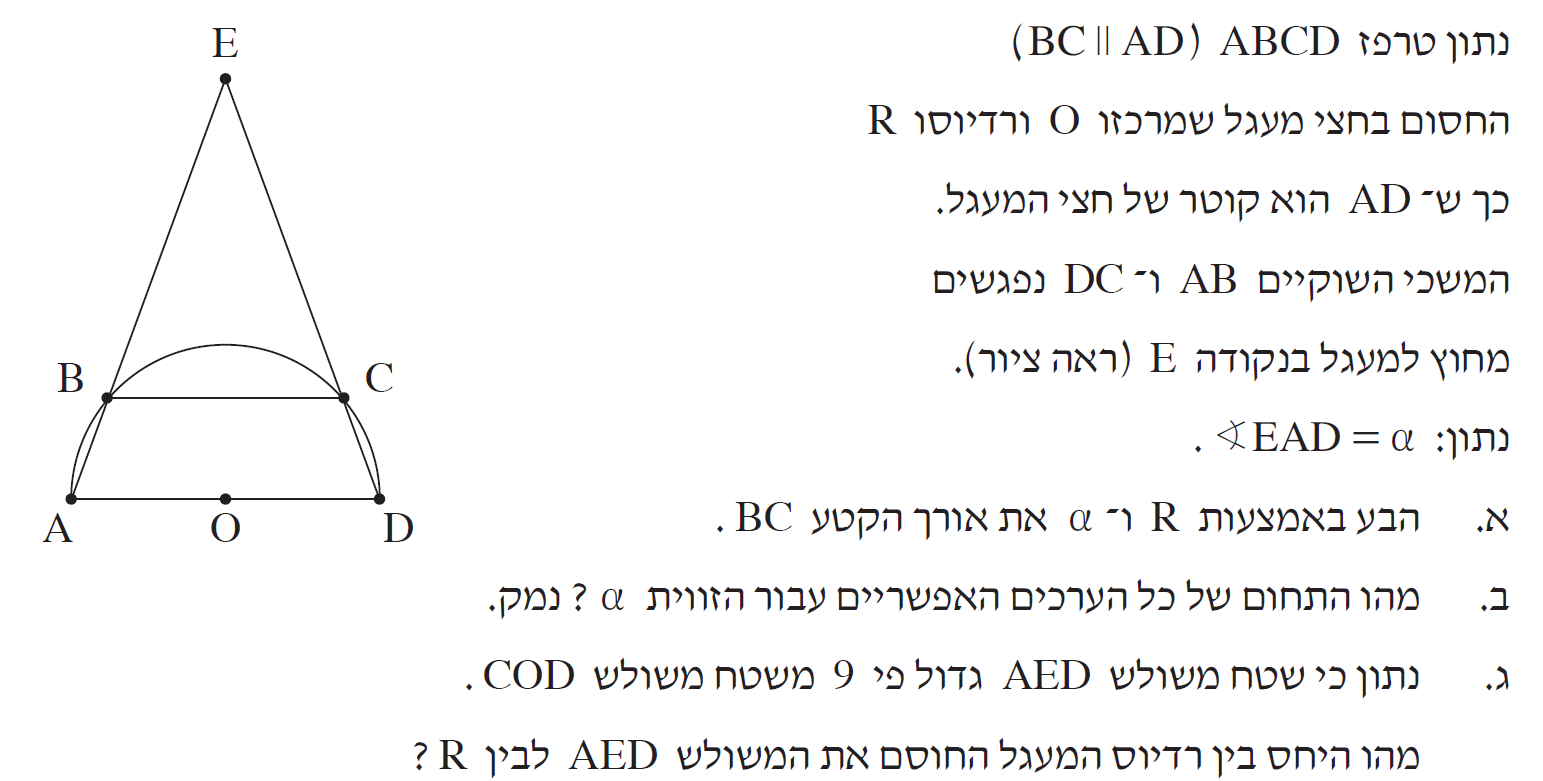
\includegraphics[width=\textwidth]{winter-2017-5}
\end{center}

\vspace{-1ex}

\textbf{סעיף א}

$OA=OB=OC=OD=R$.
נסמן זוויות לפי:

$\triangle ABO$
שווה-שוקיים, ו-%
$\angle BAO=\angle ABO=\alpha$.

כדי להשלים זוויות במשולש, ל
$180$,
$\angle AOB=180-2\alpha$,
שנסמן
$\beta$.

$\angle CBO=\beta$
לפי זוויות מתחלפות.

$\angle BCO=\beta$
כי
$\triangle BOC$
שווה-שוקיים.

נשלים זוויות של משולש ל-%
$180$
ונקבל
$\angle BOC=180-2\beta$
שנסמן 
$\gamma$.

לפי זוויות מתחלפות
$\angle COD=\beta$.

$\triangle COD$
שווה-שוקיים, ולכן
$\angle CDO=\angle OCD=(180-\beta)/2=\alpha$.

\vspace{-1ex}

\begin{center}
\selectlanguage{english}
\begin{tikzpicture}%[scale=1.1]
\coordinate (A) at (0,0);
\draw[thick] (A) -- ++(6,0) coordinate (D) -- ++(120:3) coordinate (C);
\draw[thick] (A) -- ++(60:3) coordinate (B) -- node[above] {$a$} (C);
\coordinate (O) at (3,0);
\draw[thick] (D) arc(0:180:3);
\path[name path=ae] (A) -- ($(A) ! 2.1 ! (B)$);
\path[name path=de] (D) -- ($(D) ! 2.1 ! (C)$);
\path[name intersections={of=ae and de,by={E}}];
\draw[thick] (B) -- (E) -- (C);
\fill (A) node[below left] {$A$} node[above right,xshift=4pt] {$\alpha$} circle(1.5pt);
\fill (B) node[above left] {$B$} node[below,yshift=-6pt] {$\alpha$} node[below right,xshift=8pt] {$\beta$} circle(1.5pt);
\fill (C) node[above right] {$C$} node[below,yshift=-6pt] {$\alpha$} node[below left,xshift=-8pt] {$\beta$} circle(1.5pt);
\fill (D) node[below right] {$D$}  node[above left,xshift=-4pt] {$\alpha$} circle(1.5pt);
\fill (E) node[above] {$E$} circle(1.5pt);
\fill (O) node[below] {$O$} node[above left,xshift=-8pt] {$\beta$} node[above right,xshift=8pt] {$\beta$} node[above,yshift=4pt] {$\gamma$} circle(1.5pt);
\path (O) -- node[below] {$R$} (A);
\path (O) -- node[below] {$R$} (D);
\draw[thick,dashed] (O) -- node[left,xshift=-2pt] {$R$} (B);
\draw[thick,dashed] (O) -- node[right] {$R$} (C);
\end{tikzpicture}
\end{center}

\np

נחשב
$a=BC$
לפי חוק הסינוסים ולפי חוק הקוסינוסים ב-%
$\triangle BOC$,
ותחליטו איזו שיטה עדיפה!

לפי חוק הסינוסים:

\vspace{-5ex}

\erh{12pt}
\begin{equationarray*}{rcl}
\frac{a}{\sin\gamma} &=& \frac{R}{\sin\beta}\\
a &=& \frac{R\sin(180-2\beta)}{\sin\beta} =\frac{R\sin 2\beta}{\sin\beta}\\
&=&\frac{R(2\sin \beta\cos\beta)}{\sin\beta}=2R\cos\beta = 2R\cos(180-2\alpha)\\
&=&-2R\cos 2\alpha\,.
\end{equationarray*}

\vspace{-5ex}

לפי חוק הקוסינוסים:
\erh{4pt}
\begin{equationarray*}{rcl}
a^2 &=& R^2+R^2-2R\cdot R \cos \gamma\\
&=&2R^2(1-\cos(180-2\beta)) =2R^2(1+\cos 2\beta)\\
&=&2R^2(1+\cos^2\beta-\sin^2\beta)=2R^2(2\cos^2\beta)\\
a&=&2R\cos \beta= 2R\cos(180-2\alpha)\\
&=&-2R\cos 2\alpha\,.
\end{equationarray*}

\vspace{-6ex}

\textbf{סעיף ב}

האורך של צלע חייב להיות חיובי
$a\!=\!-2R\cos 2\alpha\!>\!0$,
ולכן
$\cos 2\alpha\!<\!0$
ו-%
$2\alpha$
נמצא ברביע השני:
\begin{eqnarray*}
90<2\alpha\leq 180\\
45<\alpha\leq 90\,.
\end{eqnarray*}

\vspace{-5ex}

$\alpha \neq 90$
כי הזוויות הבסיס של משולש שווה-שוקיים חייבים להיות פחות מ-%
$90$.

\textbf{סעיף ג}

נחשב 
$S_{\triangle AED}$
לפי הנוסחה הגיאומטרית. הגובה של 
$\triangle AED$
הוא
$h=R\tan\alpha$,
ו:
\[
S_{\triangle AED}= \frac{1}{2}\cdot 2R \cdot h =R^2\tan\alpha\,.
\]

\vspace{-3ex}

נחשב 
$S_{\triangle COD}$
לפי הנוסחה הטריגונומטרית:
\erh{12pt}
\begin{equationarray*}{rcl}
S_{\triangle COD}&=&\frac{1}{2}R\cdot R \cdot \sin \beta\\
&=&\frac{1}{2}R^2 \sin (180-2\alpha)=\frac{1}{2}R^2 \sin 2\alpha\,.
\end{equationarray*}

\np

\begin{center}
\selectlanguage{english}
\begin{tikzpicture}%[scale=1.1]
\clip (-1,-.5) rectangle +(8,6.2);
\coordinate (A) at (0,0);
\draw[thick] (A) -- ++(6,0) coordinate (D) -- ++(120:3) coordinate (C);
\draw[thick] (A) -- ++(60:3) coordinate (B) -- (C);
\coordinate (O) at (3,0);
\path[name path=ae] (A) -- ($(A) ! 2.1 ! (B)$);
\path[name path=de] (D) -- ($(D) ! 2.1 ! (C)$);
\path[name intersections={of=ae and de,by={E}}];
\draw[thick] (B) -- (E) -- (C);
\fill (A) node[below left] {$A$} node[above right,xshift=4pt] {$\alpha$} circle(1.5pt);
\fill (B) node[above left] {$B$} circle(1.5pt);
\fill (C) node[above right] {$C$} circle(1.5pt);
\fill (D) node[below right] {$D$}  node[above left,xshift=-4pt] {$\alpha$} circle(1.5pt);
\fill (E) node[above] {$E$} circle(1.5pt);
\fill (O) node[below] {$O$} node[above right,xshift=8pt] {$\beta$} circle(1.5pt);
\path (O) -- node[below] {$R$} (A);
\path (O) -- node[below] {$R$} (D);
\path (O) -- node[right] {$R$} (C);
\draw[thick] (O) -- (B);
\draw[ultra thick] (O) -- (C);
\draw[ultra thick] (A) -- (E) -- (D) -- cycle;
\draw[very thick] (O) rectangle +(7pt,7pt);
\tkzCircumCenter(A,E,D)\tkzGetPoint{M}
\tkzDrawCircle[thick,dotted,name path=circle](M,A)
\draw[thick,dashed] (E) -- node[left,near start] {$h$} (O);
\end{tikzpicture}
\end{center}

לפי היחס נתון בין השטחים:
\erh{12pt}
\begin{equationarray*}{rcl}
R^2\tan\alpha &=& 9\cdot \frac{1}{2}R^2\sin 2\alpha\\
\frac{\sin\alpha}{\cos\alpha} &=& 9\cdot \frac{1}{2} \cdot 2\sin\alpha\cos\alpha\\
\cos\alpha &=& \frac{1}{3}\\
\sin\alpha &=& \sqrt{1-\left(\frac{1}{3}\right)^2} = \sqrt{\frac{8}{9}}=\frac{2\sqrt{2}}{3}\,.
\end{equationarray*}

\vspace{-2ex}

נשתמש בחוק הסינוסים כדי לחשב 
$r$,
הרדיוס של המגעל שחוסם 
$\triangle AED$:
\erh{14pt}
\begin{equationarray*}{rcl}
2r&=&\frac{DE}{\sin \alpha}\\
\cos\alpha&=&\frac{R}{DE}\\
\frac{r}{R}&=&\frac{1}{2\sin \alpha\cos\alpha}\\
&=&\frac{1}{2(2\sqrt{2}/3)(1/3)}=\frac{9}{4\sqrt{2}}=1.591\,.
\end{equationarray*}

%%%%%%%%%%%%%%%%%%%%%%%%%%%%%%%%%%%%%%%%%%%%%%%%%%%%%%%%%%%%%%

\np

\section{קיץ תשע"ו מועד ב}

\begin{center}
\selectlanguage{english}
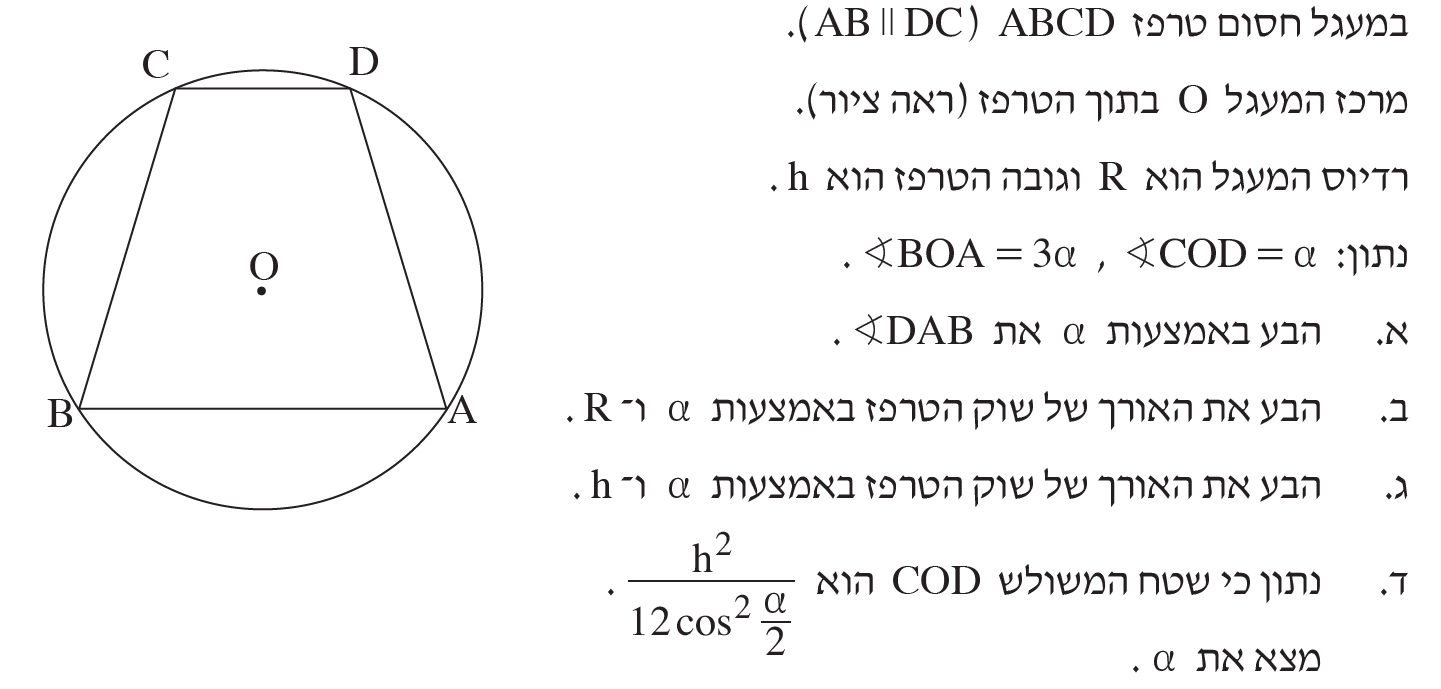
\includegraphics[width=\textwidth]{summer-2016b-5}
\end{center}

\vspace{-2ex}


מהתרשים נראה שהטרפז שווה-שוקיים, אבל אין לסמוך על תרשימים. לקח לי זמן רב עד שעלה בדעתי שטרפז חסום במעגל
\textbf{חייב}
להיות שווה-שוקיים, משפט לא מופיע ברשימת המשפטים לבגרות.בספרי לימוד המשפט לא מובלט ומופיע רק כדוגמה או תרגיל. אני אביא שתי הוכחות: אחת שלי ואחת המופיעה בספרים.

$(1)$:
$\angle ACD = \angle CAB$
לפי זוויות מתחלפות ולכן גם המיתרים הכלואים שווים
$CB=AD$.

$(2)$:
לפי משפט 
$56$
"ניתן לחסום מרובע במעגל אם ורק אם סכום זוג זוויות נגדיות שווה ל-%
$180^\circ$".
נסמן
$\angle DAB=\theta$,
ולכן 
$\angle DCB=180\!-\!\theta$.
לפי זוויות משלימות ומתאימות
$\angle DCF=\angle ABC=\theta$.
לפי משפט
$40$
"טרפז בו הזוויות שליד אותו בסיס שוות זו לזו הוא טרפז שווה-שוקיים".

\vspace{-2ex}

\begin{center}
\selectlanguage{english}
\begin{tikzpicture}[scale=.7]
\coordinate (O) at (2,1.5);
\coordinate (B) at (0,.2);
\coordinate (A) at (4,.2);
\node[draw,thick,circle through=(A),name path=circle] at (O) {};
\fill (B) node[left,xshift=-2pt] {$B$} node[above right] {$\theta$}  circle(1.5pt);
\fill (A) node[right] {$A$} circle(1.5pt);
\path[name path=bc] (B) -- +(75:4);
\path[name path=ad] (A) -- +(105:4);
\path[name intersections={of=bc and circle,by={C}}];
\path[name intersections={of=ad and circle,by={D}}];
\fill (C) node[above left] {$C$} circle(1.5pt);
\fill (D) node[above right] {$D$} circle(1.5pt);
\draw[thick] (B) -- (A) node[above left,xshift=-2pt] {$\theta$} -- (D) -- (C) node[below right,xshift=-2pt] {$180\!-\!\theta$} node[above right,xshift=2pt,yshift=2pt] {$\theta$} -- cycle;
\draw[thick] (B) -- ($(B)!1.3!(C)$) coordinate (F);
\fill (F) node[above right] {$F$} circle(1.5pt);
\end{tikzpicture}
\hspace{4em}
\begin{tikzpicture}[scale=.7]
\coordinate (O) at (2,1.5);
\coordinate (B) at (0,.2);
\coordinate (A) at (4,.2);
\node[draw,thick,circle through=(A),name path=circle] at (O) {};
\fill (B) node[left,xshift=-2pt] {$B$}  circle(1.5pt);
\fill (A) node[right] {$A$} circle(1.5pt);
\path[name path=bc] (B) -- +(75:4);
\path[name path=ad] (A) -- +(105:4);
\path[name intersections={of=bc and circle,by={C}}];
\path[name intersections={of=ad and circle,by={D}}];
\fill (C) node[above left] {$C$} circle(1.5pt);
\fill (D) node[above right] {$D$} circle(1.5pt);
\draw[thick] (B) -- (A) --(D) -- (C) -- cycle;
\draw[thick] (C) node[below right,xshift=10pt] {$\theta$} -- (A) node[above left,xshift=-10pt] {$\theta$};
\end{tikzpicture}
\end{center}

\textbf{סעיף א}

בארבעת המשולשים עם קודקוד
$O$,
הצלעות המקווקוות הם רדיוסים, כך שהמשולשים שווה-שוקיים.
$\triangle COB\cong \triangle DOA$
לפי צ.צ.צ. כי הטרפז שווה-שוקיים. מכאן ש-%
$\angle COB= \angle DOA$,
וניתן לסמן את הזוויות לפי החישובים מימין לתרשים. החישוב של
$\gamma$
מוצדק כי סכום הזוויות סביב נקודה הוא 
$360$.
השורה האחרונה מציגה את התשובה לשאלה כי
$\angle DAB=\beta+\delta$.

\selectlanguage{english}
\hspace{2em}
\begin{minipage}{.38\textwidth}
\begin{tikzpicture}%[scale=.95]
\coordinate (O) at (2,1.5);
\coordinate (B) at (0,.2);
\coordinate (A) at (4,.2);
\node[draw,thick,circle through=(A),name path=circle] at (O) {};
\fill (O) node[left,xshift=-4pt,yshift=2pt] {$\gamma$} node[below,yshift=-6pt] {$3\alpha$} node[above,yshift=10pt] {$\alpha$} node[right,xshift=6pt] {$\gamma$} circle(1.5pt);
\fill (B) node[left,xshift=-2pt] {$B$} node[above right,xshift=26pt] {$\beta$} circle(1.5pt);
\fill (A) node[right] {$A$} node[above left,xshift=-22pt] {$\beta$} node[above left,xshift=-6pt,yshift=14pt] {$\delta$} circle(1.5pt);
\path[name path=bc] (B) -- +(75:4);
\path[name path=ad] (A) -- +(105:4);
\path[name intersections={of=bc and circle,by={C}}];
\path[name intersections={of=ad and circle,by={D}}];
\fill (C) node[above left] {$C$} circle(1.5pt);
\fill (D) node[above right] {$D$} node[below left,xshift=4pt,yshift=-12pt] {$\delta$}  circle(1.5pt);
\draw[thick] (B) -- (A) --(D) -- (C) -- cycle;
\draw[thick,dashed] (O) -- (A);
\draw[thick,dashed] (O) -- (B);
\draw[thick,dashed] (O) -- (C);
\draw[thick,dashed] (O) -- (D);
\draw[very thick,dotted] (C) -- node[right,yshift=4pt] {$h$} ($(B)!(C)!(A)$) node[below] {$E$};
\draw[rotate=90] ($(B)!(C)!(A)$) rectangle +(6pt,6pt);
\end{tikzpicture}
\end{minipage}
\begin{minipage}{.47\textwidth}
\erh{12pt}
\begin{equationarray*}{rcl}
\beta &\!\!=\!\!& \frac{180\!-\!3\alpha}{2}\\
\gamma &\!\!=\!\!& \frac{360\!-\!(\alpha\!+\!3\alpha)}{2}=180\!-\!2\alpha\\
\delta &\!\!=\!\!&\frac{180\!-\!\gamma}{2}= \frac{180\!-\!(180\!-\!2\alpha)}{2}=\alpha\\
\beta\!+\!\delta&\!\!=\!\!&\frac{180\!-\!\alpha}{2}\,.
\end{equationarray*}
\end{minipage}
\selectlanguage{hebrew}

\textbf{סעיף ב}

כדי חשב אורך של שוק נחפש משולש שאחת מצלעותיו היא
$DA$.
לפי חוק בסינוסים ב-%
$\triangle DOA$:
\erh{12pt}
\begin{equationarray*}{rcl}
\frac{DA}{\sin\gamma}&=&\frac{R}{\sin\delta}\\
\frac{DA}{\sin(180\!-\!2\alpha)}&=&\frac{R}{\sin\alpha}\\
DA&=&\frac{R\sin 2\alpha}{\sin\alpha}\\
&=&\frac{R\cdot 2\sin \alpha\cos\alpha}{\sin\alpha} = 2R\cos\alpha\,.
\end{equationarray*}

\vspace{-4ex}

\textbf{סעיף ג}

בתרשים בנינו את הגובה מהנקודה 
$C$
כדי לא להסתיר את הסימונים ב-%
$\triangle DOA$.
$CB=DA$
הוא גם שוק. נשתמש בהגדרה של סינוס במשולש 
$\triangle CBE$:
\[
\frac{h}{CB}=\sin \angle CBE=\sin \left(90-\frac{\alpha}{2}\right)=\cos\frac{\alpha}{2}\,,
\]
כי
$\angle CBE=\angle DAB=\beta+\delta$.
התשובה היא
$CB=\displaystyle\frac{h}{\cos (\alpha/2)}$.

\textbf{סעיף ד}

בנוסחה הטריגונטמרית עבור
$S_{\triangle COD}$
יופיעו אורכי הצלעות
$R$
והזווית
$\alpha$.
אנו רוצים נוסחה עם 
$h$
ו-%
$\alpha$
כדי להשוות לביטוי הנתון. נשווה את הביטויים עבור שוקי הטרפז מהסעיפים הקודמים:
\erh{12pt}
\begin{equationarray*}{rcl}
2R\cos\alpha&=&\frac{h}{\cos(\alpha/2)}\\
R&=&\frac{h}{2\cos\alpha \cos(\alpha/2)}\,.
\end{equationarray*}

\np

נציב בנוסחה לשטח, נשווה לנוסחה הנתונה לשטח ונצמצם:
\erh{16pt}
\begin{equationarray*}{rcl}
\frac{h^2}{12\cos^2 (\alpha/2)}&=&\frac{1}{2}\cdot OC \cdot OD \cdot \sin\alpha=\frac{1}{2}R^2\sin\alpha\\
&=&\frac{1}{2}\cdot \frac{h^2}{4}\cdot \frac{1}{\left(\cos\alpha \cos(\alpha/2)\right)^2} \cdot \sin\alpha\\
\frac{1}{12}&=&\frac{1}{8}\cdot \frac{1}{\cos^2\alpha} \cdot \sin\alpha=\frac{1}{8}\cdot \frac{1}{1-\sin^2\alpha} \cdot \sin\alpha\\
2\sin^2\alpha + 3\sin\alpha - 2&=&(2\sin\alpha-1)(\sin\alpha+2)= 0\,.
\end{equationarray*}
נבחר את השורש 
$\sin \alpha = \displaystyle\frac{1}{2}$
כי הערך של סינוס לא יכול להיות
$-2$.

הערך היחיד ש-%
$\alpha$
יכול לקבל הוא
$30^\circ$
כי זוויות הבסיס של טרפז חייבים להיות פחות מ-%
$90^\circ$.

%%%%%%%%%%%%%%%%%%%%%%%%%%%%%%%%%%%%%%%%%%%%%%%%%%%%%%%%%%%%%%


\np

\section{קיץ תשע"ו מועד א}

\begin{center}
\selectlanguage{english}
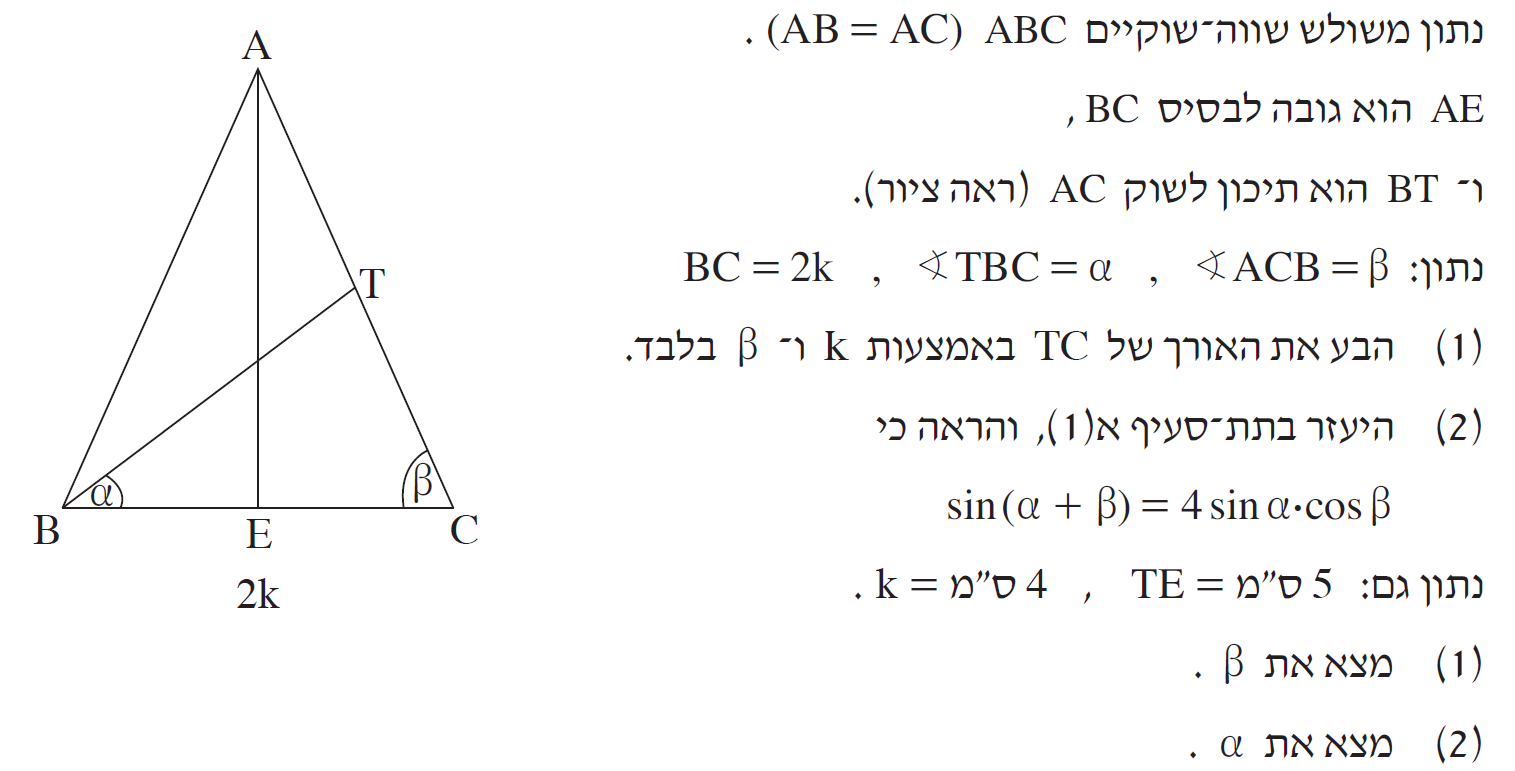
\includegraphics[width=\textwidth]{summer-2016a-5}
\end{center}

\vspace{-3ex}

\begin{center}
\selectlanguage{english}
\begin{tikzpicture}[scale=.85]
\coordinate (B) at (0,0);
\coordinate (C) at (5,0);
\path[name path=ba] (B) -- +(66:7);
\path[name path=ca] (C) -- +(114:7);
\path[name intersections={of=ba and ca,by={A}}];
\fill (A) node[above] {$A$} circle(1.5pt);
\fill (B) node[below left] {$B$} node[above right,xshift=12pt] {$\alpha$} circle(1.5pt);
\fill (C) node[below right] {$C$} node[above left,xshift=-6pt] {$\beta$} circle(1.5pt);
\coordinate (T) at ($(A)!.5!(C)$);
\fill (T) node[right] {$T$} circle(1.5pt);
\draw[thick] (B) -- (T);
\coordinate (E) at ($(B)!(A)!(C)$);
\draw[thick] (A) -- (E);
\fill (E) node[below] {$E$} circle(1.5pt);
\draw[rotate=90] (E) rectangle +(8pt,8pt);
\draw[thick] (A) -- node[left] {$2a$} (B) -- node[below] {$k$} (E) -- node[below] {$k$} (C) -- node[right] {$a$} (T) -- node[right] {$a$} (A);
\node at ($(T)+(60pt,-10pt)$) {$180\!-\!(\alpha\!+\!\beta)$};
\draw[->] ($(T)+(25pt,-9pt)$) -- +(-28pt,0);
\end{tikzpicture}
\end{center}

\vspace{-1ex}

$(1)$
לפי הגדרת הקוסינוס ב-%
$\triangle AEC$:

\vspace{-3ex}

\erh{12pt}
\begin{equationarray*}{rcl}
\cos \beta &=& \frac{k}{2a}\\
TC = a &=& \frac{k}{2\cos\beta}\,.
\end{equationarray*}

\vspace{-2ex}

$(2)$
נחפש משולש עבורו חוק הסינוסים ייתן משוואה בה יצטמצם
$k$
או
$a$.
$\triangle TBC$ 
מתאים:

\vspace{-5ex}

\selectlanguage{english}
\erh{14pt}
\begin{equationarray*}{rcl}
\frac{2k}{\sin(180\!-\!(\alpha\!+\!\beta))}&=&\frac{a}{\sin\alpha}\\
\frac{2k}{\sin(\alpha\!+\!\beta)}&=&\frac{k/(2\cos\beta)}{\sin\alpha}\\
\sin(\alpha\!+\!\beta)&=&4\sin\alpha\cos\beta\,.
\end{equationarray*}
\selectlanguage{hebrew}

\np

$\bm{(1)}$
נוסיף את אורכי הצלעות הנתונים לתרשים ונשתמש במשפט
$86$
"במשולש ישר זווית התיכון ליתר שווה למחצית היתר" כדי להסיק ש-%
$TE=\frac{1}{2}AC=5$:
\begin{center}
\selectlanguage{english}
\begin{tikzpicture}[scale=.9]
\coordinate (B) at (0,0);
\coordinate (C) at (5,0);
\path[name path=ba] (B) -- +(66:7);
\path[name path=ca] (C) -- +(114:7);
\path[name intersections={of=ba and ca,by={A}}];
\fill (A) node[above] {$A$} circle(1.5pt);
\fill (B) node[below left] {$B$} node[above right,xshift=12pt] {$\alpha$} circle(1.5pt);
\fill (C) node[below right] {$C$} node[above left,xshift=-6pt] {$\beta$} circle(1.5pt);
\coordinate (T) at ($(A)!.5!(C)$);
\fill (T) node[right] {$T$} circle(1.5pt);
\draw[thick] (B) -- (T);
\coordinate (E) at ($(B)!(A)!(C)$);
\draw[thick] (A) -- (E);
\fill (E) node[below] {$E$} node[above right,xshift=2pt] {$\beta$}circle(1.5pt);
\draw[rotate=90] (E) rectangle +(8pt,8pt);
\draw[thick] (A) -- (B) -- (C) -- node[right] {$5$} (T) -- node[right] {$5$} (A);
\coordinate (F) at ($(E)!(T)!(C)$);
\draw[thick,dashed] (E) -- node[above,xshift=-2pt] {$5$} (T) -- (F);
\path (B) -- node[below] {$4$} (E) -- node[below] {$2$} (F) -- node[below] {$2$} (C);
\draw (F) rectangle +(8pt,8pt);
\end{tikzpicture}
\end{center}

נוריד גובה מ-%
$T$
שהוא אנך אמצעי במשלוש שווה-שוקיים
$\triangle ETC$
ונקבל:
\erh{10pt}
\begin{equationarray*}{rcl}
\cos\beta &=& \frac{2}{5}\\
\beta &=&66.4^\circ\,.
\end{equationarray*}

\vspace{-4ex}

$\bm{(2)}$
לפי סעיף 
$(1)$
וסעיף 
$(2)$
הקודם:

\vspace{-5ex}

\erh{14pt}
\begin{equationarray*}{rcl}
\sin(\alpha+\beta)&=&4\sin\alpha\cos\beta\\
\sin\alpha\cos\beta+\cos\alpha\sin\beta&=&4\sin\alpha\cos\beta\\
(\sin\alpha)\cdot\frac{2}{5}+\cos\alpha\sqrt{1-\left(\frac{2}{5}\right)^2}&=&4\cdot (\sin\alpha)\cdot\frac{2}{5}\\
\sqrt{21}\cos\alpha&=&6\sin\alpha\\
\tan\alpha &=& \frac{\sqrt{21}}{6}\\
\alpha&=&37.37^\circ\,.
\end{equationarray*}

%%%%%%%%%%%%%%%%%%%%%%%%%%%%%%%%%%%%%%%%%%%%%%%%%%%%%%%%%%%%%%
\np


\section{חורף תשע"ו}

\begin{center}
\selectlanguage{english}
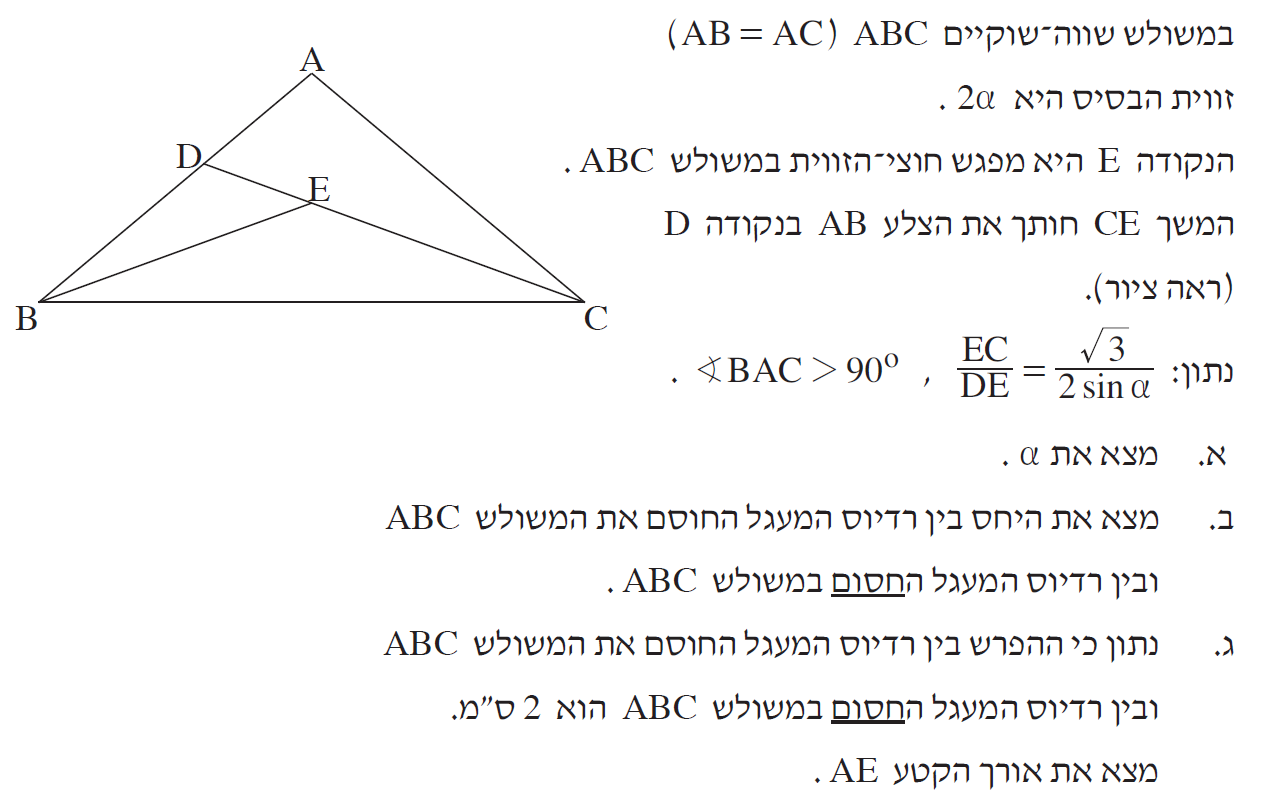
\includegraphics[width=\textwidth]{winter-2016-5}
\end{center}

\vspace{-2ex}

לפי משפט
$6$
"במשולש שווה-שוקיים , חוצה זווית הראש, התיכון לבסיס והגובה לבסיס מתלכדים", ולכן חוצה הזווית
$\angle BAC$
עובר דרך
$E$
וחוצה את
$BC$
בנקודה 
$F$
בזווית ישרה. נסמן זוויות:


$\angle FEB = \triangle FEC=90$
ולכן
$\angle BEF=\angle CEF=90\!-\!\alpha$
שנסמן 
$\beta$.

$\angle AFB=\angle AFC=90$
ולכן
$\angle BAF=\angle CAF=90\!-\!2\alpha$
שנסמן
$\gamma$.

$\angle AED=\beta$
לפי זוויות קודקודיות, ו-%
$\angle ADE=180\!-\!\beta\!-\!\gamma=3\alpha$.

$\angle BDE=180\!-\!3\alpha$
לפי זוויות משלימות.

\vspace{-	1ex}

\begin{center}
\selectlanguage{english}
\begin{tikzpicture}%[scale=1.1]
\coordinate (B) at (0,0);
\coordinate (C) at (10,0);
\path[name path=ba] (B) -- +(40:7);
\path[name path=ca] (C) -- +(140:7);
\path[name intersections={of=ba and ca,by={A}}];
\fill (A) node[above] {$A$} node[below right,xshift=0pt,yshift=-8pt] {$\gamma$} node[below left,yshift=-8pt] {$\gamma$} circle(1.5pt);
\fill (B) node[below left] {$B$} node[above right,xshift=24pt,yshift=12pt] {$\alpha$} node[above right,xshift=30pt] {$\alpha$} circle(1.5pt);
\fill (C) node[below right] {$C$} node[above left,xshift=-24pt,yshift=12pt] {$\alpha$} node[above left,xshift=-30pt] {$\alpha$} circle(1.5pt);
\draw[thick] (A) -- (B) -- (C) -- cycle;
\path[name path=cbis] (C) -- +(160:8);
\path[name path=bbis] (B) -- +(20:8);
\path[name intersections={of=ba and cbis,by={D}}];
\path[name intersections={of=bbis and cbis,by={E}}];
\fill (D) node[left] {$D$} node[right,xshift=8pt,yshift=2pt] {$3\alpha$} node[below left,xshift=-20pt] {$180\!-\!3\alpha$} circle(1.5pt);
\draw[->] ($(D)+(-22pt,-10pt)$) -- +(20pt,0);
\fill (E) node[above right] {$E$} node[above left,yshift=2pt] {$\beta$} node[below left,yshift=-4pt] {$\beta$} node[below right,yshift=-4pt] {$\beta$} node[left,xshift=-10pt] {$2\alpha$} circle(1.5pt);
\draw[thick] (C) -- (D);
\draw[thick] (B) -- node[above] {$a$} (E);
\path (C) -- node[above] {$a$} (E);
\coordinate (F) at (A |- B);
\draw[thick,dashed] (A) -- (F);
\fill (F) node[below] {$F$} circle(1.5pt);
\draw (F) rectangle +(7pt,7pt);
\node at ($(A)+(90pt,-10pt)$) {$\beta = 90\!-\!\alpha$};
\node at ($(A)+(93pt,-26pt)$) {$\gamma = 90\!-\!2\alpha$};
\path (E) -- node[right,yshift=-4pt] {$r$} (F);
\end{tikzpicture}
\end{center}


\textbf{סעיף א}

נתון היחס 
$\frac{EC}{DE}$
כתלות ב-%
$\alpha$,
ולכן נחפש משלוש שעבורו חוק הסינוסים ייתן יחס אחר כתלות ב-%
$\alpha$.
$\triangle EFB\cong \triangle EFC$
לפי צ.ז.צ, כך ש-%
$EB=EC$.
לפי חוק הסינוסים ב-%
$\triangle BDE$:

\np

\erh{14pt}
\begin{equationarray*}{rcl}
\frac{EB}{\sin(180\!-\!3\alpha)}&=&\frac{DE}{\sin\alpha}\\
\frac{EB}{DE}&=&\frac{\sin(180\!-\!3\alpha)}{\sin\alpha}=\frac{\sin 3\alpha}{\sin\alpha}= \frac{\sqrt{3}}{2\sin\alpha}\\
\sin 3\alpha&=&\frac{\sqrt{3}}{2}\,.
%\alpha&=&20^\circ\,.
\end{equationarray*}
הפתרונות הם 
$\alpha=20^\circ, \alpha=40^\circ$,
אבל נבחר
$\alpha=20^\circ$,
כי אם
$\alpha=40^\circ$,
$\angle BAC=20^\circ$
הסותר את הנתון
$\angle BAC > 90^\circ$.


\textbf{סעיף ב}

לפי משפט
$49$
"שלושת חוצי הזוויות של משולש נחתכים בנקודה אחת, שהיא מרכז המעגל החסום במשולש",
$E$
היא מרכז המעגל החסום שמשיק לצלע המשולש ב-%
$F$,
ו-%
$r=EF$
הוא הרדיוס.

צריך להיזהר שלא לקבוע ש-%
$E$
היא מרכז המעגל החוסם כי אין אנו יודעים שחוצי הזוויות האחרות הם גם אנכים אמצעיים. במקום זה נשתמש בחוק הסינוסים על המשלוש
$\triangle ABC$.
נבחר את הזווית
$\angle BAC=180\!-\!4\alpha$,
כי אפשר לחשב את אורך הצלע הנגדית
$BC$
כתלות ב-%
$r,\alpha$:

\vspace{-4ex}
\erh{14pt}
\begin{equationarray*}{rcl}
\tan\alpha &=& \frac{r}{BF}=\frac{r}{BC/2}\\ 
2R&=&\frac{BC}{\sin (180\!-\!4\alpha)}=\frac{2r}{\sin 4\alpha\tan\alpha}\\
\frac{R}{r}&=&\frac{1}{\sin 4\alpha\cdot\tan \alpha}=\frac{1}{\sin 80\cdot\tan 20}=2.79\,.
\end{equationarray*}

\vspace{-2ex}

\textbf{סעיף ג}

נתון
$R-r=2$.
נציב 
$R=2.79r$
שחישבנו בסעיף ב, ונקבל
$r=2/(2.79-1)=1.117$.

אין לנו מספיק מידע על המשולש
$\triangle AED$,
ולכן נחשב עם
$AF=AE+EF=AE+r$:
\erh{14pt}
\begin{equationarray*}{rcl}
\tan 2\alpha&=&\frac{AF}{BF}=\frac{AE+r}{r/\tan\alpha}\\
AE&=&\frac{r(\tan 2\alpha - \tan \alpha)}{\tan \alpha}\\
&=&\frac{1.117(\tan 40-\tan 20)}{\tan 20}=1.458\,.
\end{equationarray*}

%%%%%%%%%%%%%%%%%%%%%%%%%%%%%%%%%%%%%%%%%%%%%%%%%%%%%%%%%%%%%%


\np

\section{קיץ תשע"ה מועד ב}

\begin{center}
\selectlanguage{english}
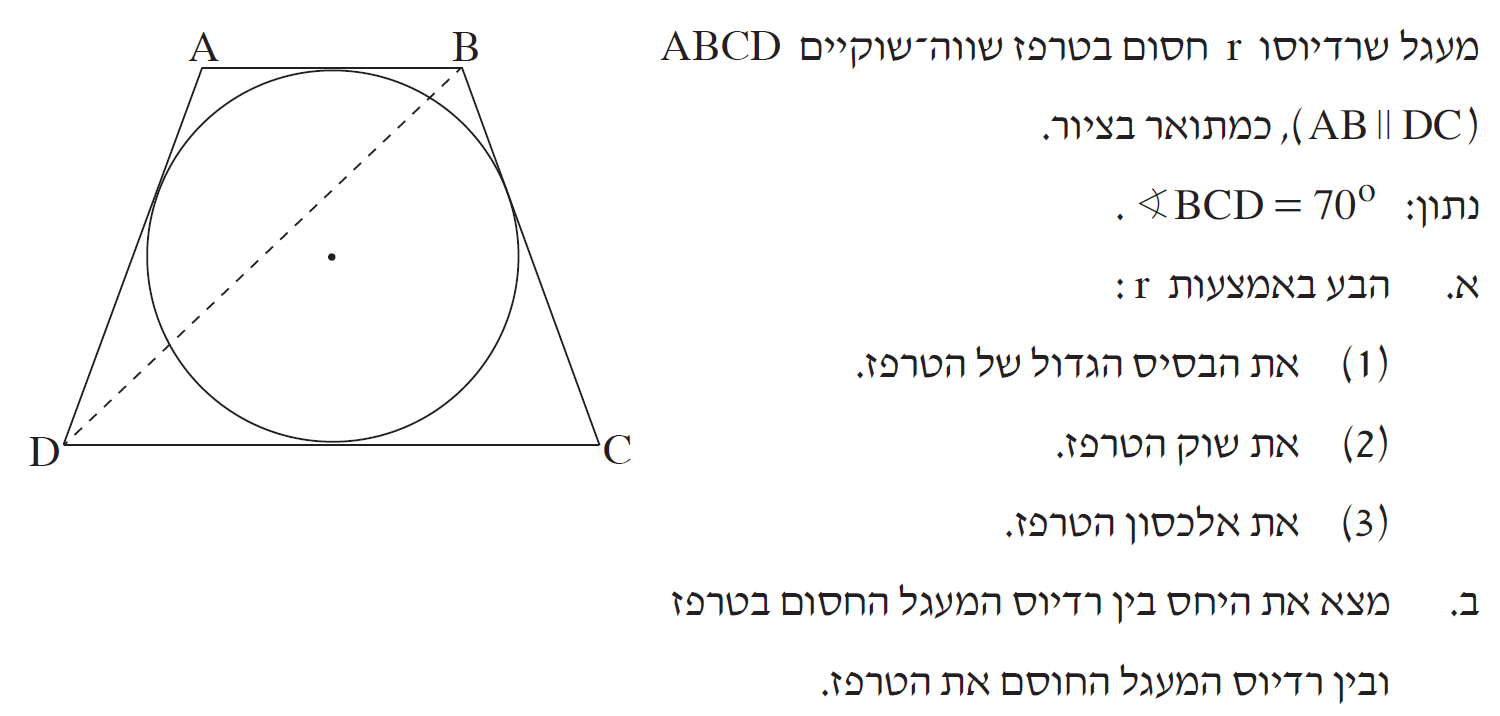
\includegraphics[width=\textwidth]{summer-2015b-5}
\end{center}
נוריד אנך מ-%
$A$
שחתוך את
$DC$
ב-%
$G$,
ואנך מ-%
$B$
שחותך את 
$DC$
ב-%
$H$.
בטרפז
$AB\|DC$
ולכן
$ABHG$
הוא מלבן. לפי משפט
$77$
"המשיק למעגל מאונך לרדיוס בנקודת ההשקה", האנך מנקודת ההשקה של מעגל עם
$AB$
עובר דרך מרכז המעגל והוא ניצב לנקודת ההשקה עם
$DC$.
מכאן ש-%
$AG=EF=BF=2r$.

נסמן
$AB=GH=b_2$.
הטרפז שווה-שוקיים ולפי משפט
$39$
"בטרפז שווה-שוקיים הזוויות שליד אותו בסיס שוות זו לזו",
$\angle ADC=70^\circ$,
ו-%
$\angle DAG=\angle CBH=20^\circ$
כדי להשלים ל-%
$180$
במשולש. ביחד עם 
$AD=BC$
בטרפז שווה-שוקיים,
$\triangle ADG \cong \triangle BCH$.
נסמן
$DG=HC=b_1$
ונקבל ש-%
$DC=2b_1+b_2$
שנסמן
$b$.

\begin{center}
\selectlanguage{english}
\begin{tikzpicture}
\node[circle,draw,thick] (In) at (0,0) [minimum size=5cm] {};
\coordinate (D) at (-3.5,-2.5);
\draw[thick] (D) -- +(7,0) coordinate (C) node[above left,xshift=-2pt] {$70$};
\fill (C) node[below right] {$C$} circle(1.5pt);
\fill (D) node[below left] {$D$}  node[above right,xshift=2pt] {$70$} circle(1.5pt);
\coordinate (DA) at (tangent cs:node=In,point={(D)},solution=2);
\path[name path=da] (D) -- ($(D)!1.7!(DA)$);
\fill (DA) circle(1.5pt);
\coordinate (CB) at (tangent cs:node=In,point={(C)},solution=1);
\path[name path=cb] (C) -- ($(C)!1.7!(CB)$);
\fill (CB) circle(1.5pt);
\path[name path=top] (-3,2.5) -- (3,2.5);
\path[name intersections={of=da and top,by={A}}];
\path[name intersections={of=cb and top,by={B}}];
\fill (A) node[above left] {$A$} circle(1.5pt);
\fill (B) node[above right] {$B$} circle(1.5pt);
\draw[thick] (D) -- node[left] {$s$} (A) -- (B) -- node[right] {$s$} (C);
\draw[thick,dashed] (D) -- (B);
\coordinate (G) at ($(D)!(A)!(C)$);
\draw[thick,dashed] (A) -- node[right,yshift=8pt] {$2r$} (G);
\fill (G) node[below,yshift=-1pt] {$G$} circle(1.5pt);
\coordinate (H) at ($(D)!(B)!(C)$);
\draw[thick,dashed] (B) -- node[left,yshift=8pt] {$2r$} (H);
\fill (H) node[below,yshift=-1pt] {$H$} circle(1.5pt);
\draw (G) rectangle +(8pt,8pt);
\draw (H) rectangle +(8pt,8pt);
\coordinate (E) at ($(A)!.5!(B)$);
\fill (E) node[above] {$E$} circle(1.5pt);
\coordinate (F) at ($(D)!(E)!(C)$);
\fill (F) node[below] {$F$} circle(1.5pt);
\draw[thick,dashed] (E) -- node[right,yshift=8pt] {$2r$} (F);
\draw (F) rectangle +(8pt,8pt);
\draw[<->] ($(D)+(0,-8mm)$) -- node[fill=white] {$b_1$} ($(G)+(0,-8mm)$);
\draw[<->] ($(G)+(0,-8mm)$) -- node[fill=white] {$b_2$} ($(H)+(0,-8mm)$);
\draw[<->] ($(H)+(0,-8mm)$) -- node[fill=white] {$b_1$} ($(C)+(0,-8mm)$);
\draw[<->] ($(D)+(0,-14mm)$) -- node[fill=white] {$b$} ($(C)+(0,-14mm)$);
\draw[<->] ($(A)+(0,8mm)$) -- node[fill=white] {$b_2$} ($(B)+(0,8mm)$);
\end{tikzpicture}
\end{center}

\np

\textbf{סעיף א}

$(1)$
נחפש משפט הקושר צלעות של מרובע עם הרדיוס של המעגל החסום. משפט
$57$
"מרובע קמור חוסם מעגל אם ורק אם סכום שתי צלעות נגדיות שווה לסכום שתי הצלעות הנגדיות האחרות":
\[
2s=b+b_2=(b_1+b_2+b_1)+b_2=2(b_1+b_2)\,.
\]
ממשוואה זו נחשב משוואות נוספות שיעזרו לנו בהמשך:
\[
s=b_1+b_2,\quad b=2b_1+b_2=s+b_1\,.
\]
לפי ההגדרות של הפונקציות הטריגונומרטיות ב-%
$\triangle ADC$,
נוכל לקשר את 
$r$
לצלעות:
\erh{12pt}
\begin{equationarray*}{rcl}
\tan 70 &=& \frac{2r}{b_1}\\
\sin 70&=&\frac{2r}{s}\\
b&=&s+b_1\\
&=&2r\left(\frac{1}{\sin 70}+\frac{1}{\tan 70}\right)=2.856r\,.
\end{equationarray*}

\vspace{-3ex}

$(2)$
$s=\displaystyle\frac{2r}{\sin 70}=2.128r$.

\medskip

$(3)$
האלכסון הוא היתר של 
$\triangle BDH$
שצלעותיו ידועות:

\vspace{-6ex}

\erh{20pt}
\begin{equationarray*}{rcl}
DB^2&=& (b_1+b_2)^2 + (2r)^2=s^2 +(2r)^2\\
&=& \left(\frac{2r}{\sin 70}\right)^2 + 4r^2\\
DB&=&2r\sqrt{\left(\frac{1}{\sin 70}\right)^2+1}=2.921r\,.
\end{equationarray*}

\vspace{-3ex}

\textbf{סעיף ב}

במבט ראשון נראה שכדאי להשתמש במשפט
$56$
"ניתן לחסום מרובע במעגל אם ורק אם סכום זוג זוויות נגדיות שווה ל-%
$180^\circ$",
אבל אין בו צורך. שימו לב שהמרכז של המעגל החוסם לא חופף את המרכז של המעגל החסום, כך שאי-אפשר לחשב 
$R$,
הרדיוס של המעגל החסום, כמרחק ממרכז המעגל החוסם לאחד מקודקודי הטרפז. במקום זה נשתמש בחוק הסינוסים ב-%
$\triangle BCD$:
\erh{16pt}
\begin{equationarray*}{rcl}
2R&=&\frac{DB}{\sin BCD}=\frac{2.921r}{\sin 70}\\
\frac{r}{R}&=&\frac{2\cdot \sin 70}{2.921}=6.434\,.
\end{equationarray*}

%%%%%%%%%%%%%%%%%%%%%%%%%%%%%%%%%%%%%%%%%%%%%%%%%%%%%%%%%%%%%%

\np

\section{קיץ תשע"ה מועד א}

\begin{center}
\selectlanguage{english}
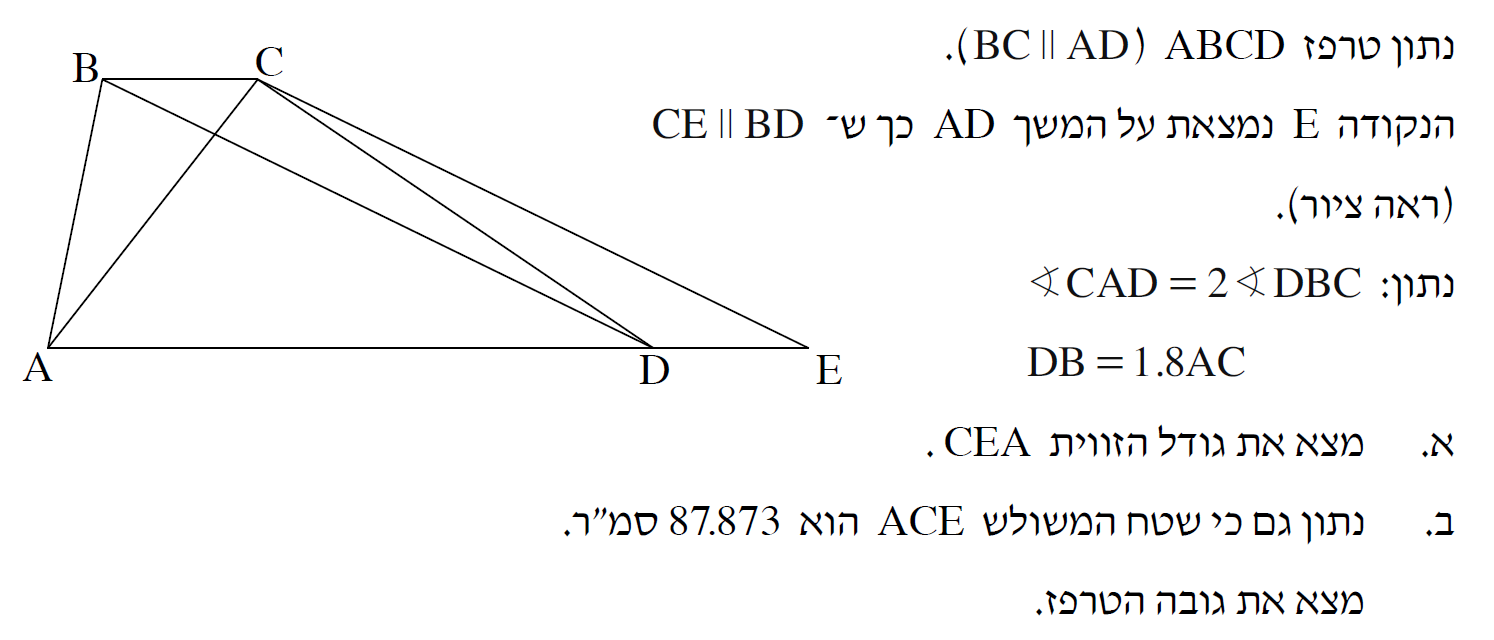
\includegraphics[width=\textwidth]{summer-2015a-5}
\end{center}

\vspace{-1ex}

\textbf{סעיף א}

נסמן זוויות לפי זוויות מתחלפות, מתאימות ופנימיות:
$\angle CBD=\angle BDA=\angle CEA=\alpha$,
$\angle BCE=\angle BDE=180-\alpha$.

\vspace{-2ex}

\begin{center}
\selectlanguage{english}
\begin{tikzpicture}[scale=1.2]
\draw[thick] (0,0) coordinate (A) node[below left] {$A$} -- (6,0) coordinate (D) node[below] {$D$} -- (8,0) coordinate (E) node[below right] {$E$} -- (3,3) coordinate (C) node[above right] {$C$} -- (1,3) coordinate (B) node[above left] {$B$} -- (A) -- node[above,xshift=-2pt] {$a$} (C);
\draw[thick] (B) -- node[below,xshift=-2pt] {$1.8a$} (D) -- (C);
\fill (A) node[above right,xshift=12pt] {$2\alpha$} circle(1.5pt);
\fill (B) node[below right,xshift=16pt] {$\alpha$} circle(1.5pt);
\fill (C) circle(1.5pt);
\fill (D) node[above left,xshift=-16pt] {$\alpha$} circle(1.5pt);
\fill (E) node[above left,xshift=-16pt] {$\alpha$} circle(1.5pt);
\draw[ultra thick] (A) -- (E) -- node[above,xshift=4pt,yshift=2pt] {$1.8a$} (C) -- cycle;
\draw ($(D)+(6mm,0)$) arc[start angle=0,end angle=150,radius=6mm];
\node at ($(E)+(-6pt,30pt)$) {$180\!-\!\alpha$};
\draw[->] ($(E)+(-6pt,25pt)$) -- +(-35pt,-12pt);
\draw ($(C)+(-6mm,0)$) arc[start angle=180,end angle=330,radius=6mm];
\node at ($(C)+(40pt,-4pt)$) {$180\!-\!\alpha$};
\draw[->] ($(C)+(40pt,-8pt)$) -- +(-40pt,-4pt);
\end{tikzpicture}
\end{center}

\vspace{-1ex}

לפי חוק הסינוסים:
\vspace{-3ex}

\erh{12pt}
\begin{equationarray*}{rcl}
\frac{AC}{\sin \alpha}&=&\frac{CE}{\sin 2\alpha}\\
\frac{a}{\sin \alpha} &=& \frac{1.8a}{\sin 2\alpha}=\frac{1.8a}{2\sin \alpha\cos\alpha}\\
\cos \alpha &=& 0.9\\
\alpha &=& 25.84\,.
\end{equationarray*}

\vspace{-4ex}

\textbf{סעיף ב}

מהתרשים אפשר לראות ש-%
$S_{\triangle ACE}$
מורכב מסכום השטחים של שני משולשים עם אותו גובה:

\begin{center}
\selectlanguage{english}
\begin{tikzpicture}[scale=1.2]
\draw[thick] (0,0) coordinate (A) node[below left] {$A$} -- (8,0) coordinate (E) node[below right] {$E$} -- (3,3) coordinate (C) node[above right] {$C$} -- (1,3) coordinate (B) node[above left] {$B$} -- (A) -- node[above,xshift=-2pt] {$a$} (C);
\fill (A) node[above right,xshift=12pt] {$2\alpha$} circle(1.5pt);
\fill (B) circle(1.5pt);
\fill (C) circle(1.5pt);
\fill (E) node[above left,xshift=-16pt] {$\alpha$} circle(1.5pt);
\draw[thick] (A) -- (E) -- node[right,xshift=2pt,yshift=2pt] {$1.8a$} (C) -- cycle;
\coordinate (F) at ($(A)!(C)!(E)$);
\draw[thick,dashed] (C) -- node[left] {$h$} (F);
\fill (F) circle(1.5pt);
\draw (F) rectangle +(8pt,8pt);
\path (A) -- node[below] {$b_1$} (F) -- node[below] {$b_2$} (E);
\end{tikzpicture}
\end{center}

\vspace{-6ex}

\erh{12pt}
\begin{equationarray*}{rcl}
S_{\triangle ACE} &=& \frac{1}{2}(b_1+b_2)h\\
b_1&=& \frac{h}{\tan 2\alpha }\\
b_2&=& \frac{h}{\tan \alpha }\\
S_{\triangle ACE} &=& \frac{1}{2}h^2\left(\frac{1}{\tan 2\alpha}+\frac{1}{\tan \alpha}\right)\\
87.873 &=& \frac{1}{2}h^2(6.79+2.06) =  1.428 h^2\\
h&=& 7.846\,.
\end{equationarray*}
פתרון אחר משתמש בנוסחה הטריגונומטרית לשטח:
\erh{12pt}
\begin{equationarray*}{rcl}
S_{\triangle ACE} &=& \frac{1}{2}\cdot AC \cdot CE \cdot \sin \angle ACE\\
&=& \frac{1}{2}\cdot a \cdot 1.8a \cdot \sin (180-3\alpha)=0.9a^2\sin 3\alpha\\
87.873 &=& 0.87873 a^2\\
a&=&10\\
h &=& a\sin 2\alpha = 7.846\,.
\end{equationarray*}

%%%%%%%%%%%%%%%%%%%%%%%%%%%%%%%%%%%%%%%%%%%%%%%%%%%%%%%%%%%%%%


\np


\section{חורף תשע"ה}

\begin{center}
\selectlanguage{english}
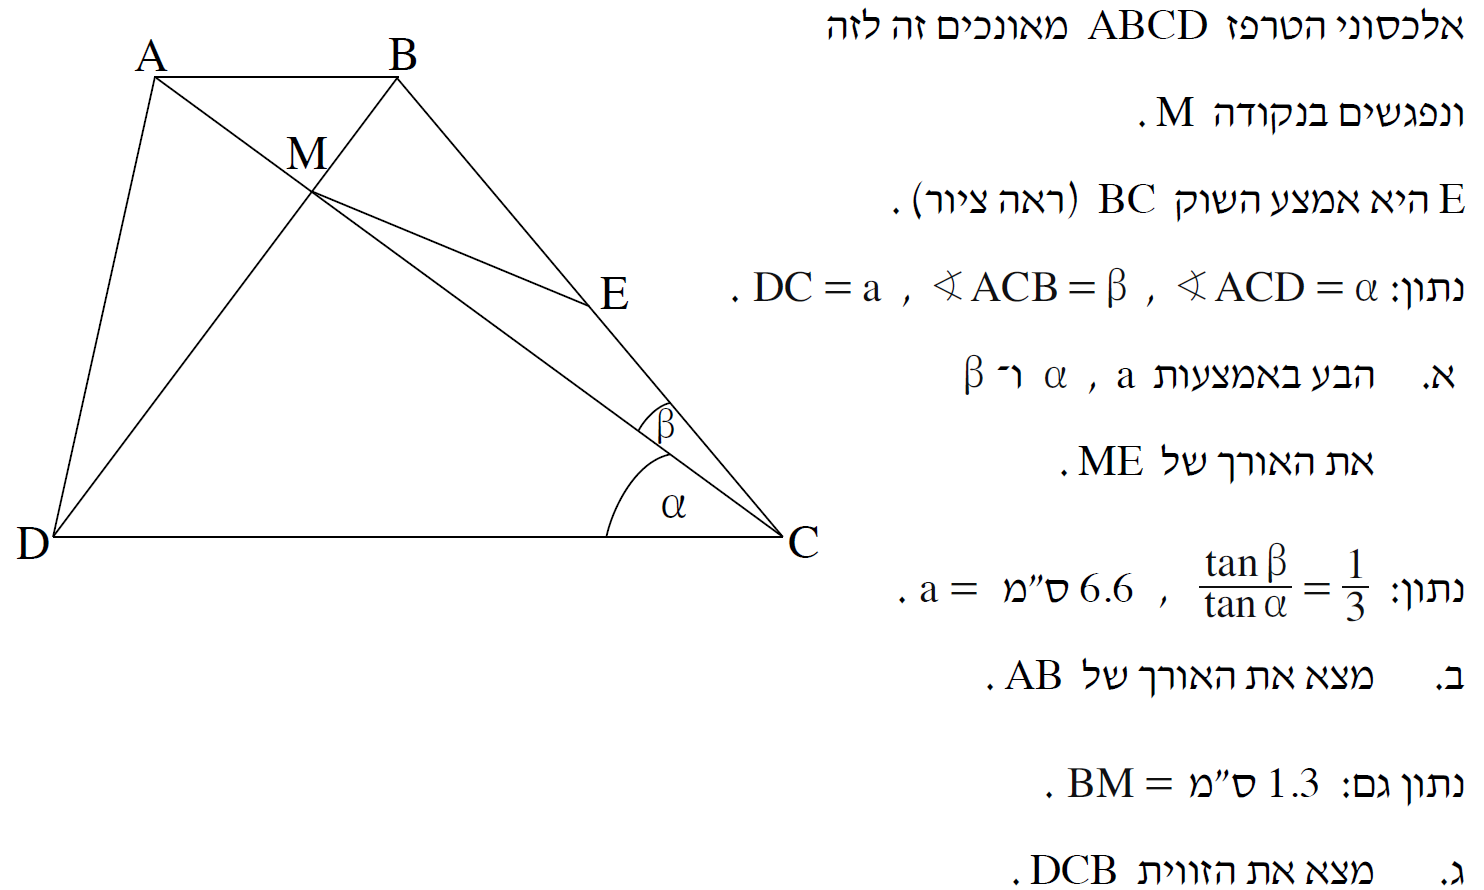
\includegraphics[width=.85\textwidth]{winter-2015-5}
\end{center}

\vspace{-1ex}

\begin{center}
\selectlanguage{english}
\begin{tikzpicture}[scale=1.1]
\draw[thick] (0,0) coordinate (D) node[left] {$D$} -- node[below] {$a$} (6,0) coordinate (C) node[right] {$C$};
\draw[thick,name path=ca] (C) -- +(144:7) coordinate (A) node[left] {$A$};
\draw[thick,name path=db] (D) -- +(54:5.1) coordinate (B) node[right] {$B$};
\draw[thick] (D) -- (A) -- node[above] {$d$} (B) -- (C);
\path[name intersections={of=ca and db,by=M}];
\fill (A) node[below right,xshift=10pt] {$\alpha$} circle(1.5pt);
\fill (B) circle(1.5pt);
\fill (C) node[above left,xshift=-12pt] {$\alpha$} node[above left,xshift=-29pt,yshift=28pt] {$\beta$}  circle(1.5pt);
\fill (D) circle(1.5pt);
\fill (M) node[left,xshift=-2pt,yshift=-2pt] {$M$} circle(1.5pt);
\draw[rotate=-126] (M) rectangle +(8pt,8pt);
\coordinate (E) at ($(B) ! .5 ! (C) $);
\fill (E) node[right] {$E$} circle(1.5pt);
\draw[thick] (M) -- node[above] {$c/2$} (E);
\path (B) -- node[right] {$c/2$} (E) -- node[right] {$c/2$} (C);
\path (M) -- node[below] {$b$} (C);
\path (M) -- node[above] {$e$} (B);
\path (D) -- node[above] {$f$} (M);
\end{tikzpicture}
\end{center}

\vspace{-2ex}

\textbf{סעיף א}

$\triangle BMC$
ישר זווית ונתון ש-%
$ME$
הוא תיכון ליתר. לפי משפט 
$86$
"במשולש ישר זווית התיכון ליתר שווה למחצית היתר",
$ME=c/2$.
לפי ההגדרות של הפונקציות הטריגונומרטיות:

\vspace{-6ex}

\erh{12pt}
\begin{equationarray*}{rcl}
\cos \beta &=& \frac{b}{c}\\
\cos \alpha &=& \frac{b}{a}\\
ME &=& \frac{c}{2} = \frac{b}{2\cos\beta}\\
&=& \frac{a\cos\alpha}{2\cos\beta}\,.
\end{equationarray*}

\np

\textbf{סעיף ב}

למשולשים
$\triangle AMB, \triangle CMB$
צלע משותפת
$MB=e$.
לפי ההגדרות של הפונקציות הטריגונומרטיות:

\vspace{-4ex}

\erh{12pt}
\begin{equationarray*}{rcl}
\tan \beta &=& \frac{e}{b}\\
\sin \alpha &=& \frac{e}{d}\\
AB = d &=& \frac{e}{\sin\alpha}=\frac{b\tan \beta}{\sin\alpha}\\
&=& \frac{a \cos\alpha\tan\beta}{\sin\alpha}=\frac{a\tan\beta}{\tan\alpha}= 6.6\cdot\frac{1}{3} = 2.2\,.
\end{equationarray*}

\vspace{-3ex}

הוכחת אחרת משתמשת במשולשים דומים. 
$\angle BAM = \angle MCD = \alpha$
לפי זוויות מתחלפות ו-%
$\triangle ABM \sim \triangle DMC$
לפי ז.ז.:

\vspace{-6ex}


\erh{12pt}
\begin{equationarray*}{rcl}
\tan \beta &=& \frac{e}{b}\\
\tan \alpha &=& \frac{f}{b}\\
\frac{e}{f}&=&\frac{\tan \beta}{\tan \alpha} =\frac{1}{3}\\
\frac{d}{a}&=& \frac{e}{f} =\frac{1}{3}\\
AB = d&=& \frac{6.6}{3}=2.2\,.
\end{equationarray*}

\vspace{-4ex}

\textbf{סעיף ג}

ממשפט פיתגורס
$b= \sqrt{a^2-f^2}=5.32$,
ו:
\erh{12pt}
\begin{equationarray*}{rcl}
\tan \beta &=& \frac{e}{b} = \frac{1.3}{5.32}=0.2444\\
\beta &=& 13.73\\
\tan \alpha &=& 3\tan\beta = 0.7331\\
\alpha &=& 36.24\\
\angle DCB &=& \alpha + \beta = 49.97\,.
\end{equationarray*}



%%%%%%%%%%%%%%%%%%%%%%%%%%%%%%%%%%%%%%%%%%%%%%%%%%%%%%%%%%%%%%

\np

\section{קיץ תשע"ד מועד ב}

\begin{center}
\selectlanguage{english}
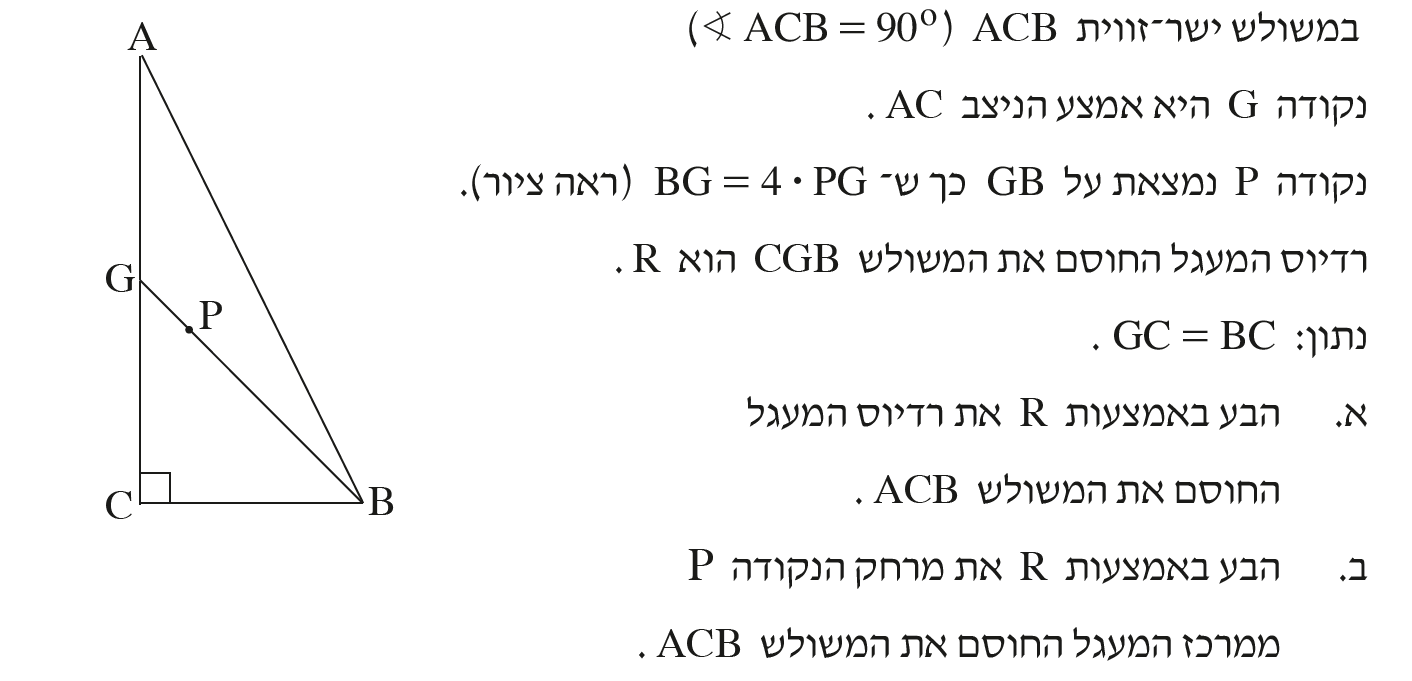
\includegraphics[width=\textwidth]{summer-2014b-5}
\end{center}

\vspace{-2ex}


נסמן
$=R,M$
מרכז המעגל החוסם את
$\triangle CGB$
והרדיוס שלו, ו-%
$=R',M'$
מרכז המעגל החוסם את
$\triangle ACB$
והרדיוס שלו. שימו לב שבתרשים הנקודות
$M,M'$
נמצאות על הצלעות
$GB, AB$,
אבל אנו חייבים להוכיח את הטענות הללו אם רוצים להשתמש בהן.
\begin{center}
\selectlanguage{english}
\begin{tikzpicture}[scale=.75]
\draw[thick] (0,0) coordinate (C) -- node[below] {$a$} (4,0) coordinate (B) -- (0,8) coordinate (A) -- cycle;
\coordinate (G) at (0,4);
\path (C) -- node[left] {$a$} (G) -- node[left] {$a$} (A);
\draw[thick] (B) -- (G);
\coordinate (P) at ($(G)!.25!(B)$);
\fill (B) node[right] {$B$} circle(1.5pt);
\fill (A) node[above] {$A$} circle(1.5pt);
\fill (C) node[left] {$C$} circle(1.5pt);
\fill (G) node[left] {$G$} circle(1.5pt);
\fill (P) node[above,yshift=2pt] {$P$} circle(1.5pt);
\tkzCircumCenter(A,B,C)\tkzGetPoint{M1}
\tkzDrawCircle[thick,dotted,name path=circle](M1,A)
\tkzCircumCenter(C,G,B)\tkzGetPoint{M2}
\tkzDrawCircle[thick,dotted,name path=circle](M2,B)
\fill (M1) node[right] {$M'$} circle(1.5pt);
\fill (M2) node[left] {$M$} circle(1.5pt);
\draw (C) rectangle +(8pt,8pt);
\end{tikzpicture}
\end{center}

\vspace{-14ex}


\textbf{סעיף א}

נשתמש בחוק הסינוסים ובמשפט פיתגורס, תחילה עבור
$\triangle CGB$:
\[
R=\frac{BG}{2\sin 90}=\frac{\sqrt{a^2+a^2}}{2}=\frac{a}{\sqrt{2}}\,,
\]
ואחר כך עבור
$\triangle ACB$:
\[
R'=\frac{AB}{2\sin 90}=\frac{\sqrt{a^2+(2a)^2}}{2}=\left(\frac{\sqrt{5}}{2}\right)a=\left(\frac{\sqrt{5}}{2}\right)\sqrt{2}R=\sqrt{\frac{5}{2}}R\,.
\]

\np

\textbf{סעיף ב}

$M'$,
מרכז המעגל החוסם את
$\triangle ACB$,
הוא נקודת החיתוך של האנכים
$GM'$
ו-%
$M'H$.


\begin{center}
\selectlanguage{english}
\begin{tikzpicture}[scale=1.3]
\clip (-.5,-1) rectangle +(5,5.4);
\draw[thick] (0,0) coordinate (C) -- (4,0) coordinate (B) -- (0,8) coordinate (A) -- cycle;
\coordinate (G) at (0,4);
\path (C) -- node[left] {$a$} (G) -- node[left] {$a$} (A);
\draw[thick] (B) -- (G);
\coordinate (P) at ($(G)!.25!(B)$);
\fill (B) node[right] {$B$} circle(1.5pt);
\fill (A) node[above] {$A$} circle(1.5pt);
\fill (C) node[left] {$C$} circle(1.5pt);
\fill (G) node[left] {$G$} circle(1.5pt);
\fill (P) node[below,xshift=-2pt,yshift=-2pt] {$P$} circle(1.5pt);
\tkzCircumCenter(A,B,C)\tkzGetPoint{M1}
\tkzCircumCenter(C,G,B)\tkzGetPoint{M2}
\fill (M1) node[right] {$M'$} circle(1.5pt);
\fill (M2) node[left,xshift=-2pt,yshift=-2pt] {$M$} circle(1.5pt);
\draw (C) rectangle +(7pt,7pt);
\draw (G) rectangle +(7pt,7pt);
\draw[thick] (P) -- node[above,xshift=-2pt] {$z$} (M1);
\coordinate (H) at (M1 |- B);
\fill (H) node[below] {$H$} circle(1.5pt);
\draw[thick,dashed] (G) -- (M1) -- (H);
\draw (H) rectangle +(7pt,7pt);
\path (G) -- node[below,xshift=-4pt,yshift=2pt] {$x$} (P) -- node[below,xshift=-4pt,yshift=2pt] {$x$} (M2) -- node[below,xshift=-4pt,yshift=2pt] {$2x$} (B);
\path (C) -- node[below] {$a/2$} (H) -- node[below] {$a/2$} (B);
\path (M1) -- node[right] {$y$} (M2) -- node[left] {$a/2$} (H);
\end{tikzpicture}
\end{center}

\vspace{-5ex}

אם נמצא משולש שעבורו נוכל לחשב שתי צלעות והזווית הכלואה ביניהן, נוכל להשתמש בחוק הקוסינוסים. ננסה את
$\triangle MPM'$.
$CG\|MH$
ולכן לפי משפט 
$91$
"משפט תאלס המורחב: ישר המקביל לאחת מצלעות המשולש חותך את שתי הצלעות האחרות או את המשכיהן בקטעים פרופורציוניים":
\[
\frac{GC}{MH}=\frac{CB}{HB}=\frac{a}{a/2}=2\,,
\]
ו-%
$MH=\displaystyle\frac{a}{2}$.
אבל
$GCHM'$
הוא מלבן, ולכן:
\[
y=MM'=M'H-MH=GC-MH=a-\frac{a}{2}=\frac{a}{2}=\frac{1}{2}\cdot \sqrt{2}R=\frac{R}{\sqrt{2}}\,.
\]
שוב לפי משפט תאלס המורחב:
\erh{12pt}
\begin{equationarray*}{rcl}
\frac{GB}{MB}&=&\frac{GC}{MH}=2\\
GB&=&GM+MB\\
GM&=&GB-MB=2MB-MB=MB\,.
\end{equationarray*}
שנסמן
$GM=MB=2x$.

נתון
$GB=4\cdot PG$,
כך ש-%
$PG=\displaystyle\frac{1}{4} (2x+2x)=x$.
לבסוף,
$PM=4x-(2x)-x=x$.
את
$x$
ניתן לחשב לפי משפט פיתגורס ב-%
$\triangle CGB$:

\vspace{-6ex}

\erh{12pt}
\begin{equationarray*}{rcl}
(4x)^2&=&a^2+a^2\\
x&=&\frac{1}{\sqrt{8}}a=\frac{1}{\sqrt{8}}\cdot\sqrt{2}R=\frac{R}{2}\,.
\end{equationarray*}

$\triangle MHB$
הוא משלוש ישר-זווית שווה-שוקיים, כך ש-%
$\angle BMH=45$,
ו-%
$\angle PMM'=45$
לפי זוויות קודקודיות. כעת יש לנו מספיק נתונים להשתמש בחוק הקוסינוסים. נסמן
$PG=z$:

\np

\erh{14pt}
\begin{equationarray*}{rcl}
z^2&=&x^2+y^2-2xy\cos \angle PMM'\\
&=&\left(\frac{R}{2}\right)^2+\left(\frac{R}{\sqrt{2}}\right)^2 - 2\left(\frac{R}{2}\right)\left(\frac{R}{\sqrt{2}}\right)\cos 45\\
&=& R^2\left(\frac{1}{4}+\frac{1}{2}-\frac{1}{\sqrt{2}}\cdot \frac{\sqrt{2}}{2}\right)=\frac{R^2}{4}\\
z&=&\frac{R}{2}\,.
\end{equationarray*}

\vspace{-4ex}

\begin{center}
*\ *\ *
\end{center}

פתרון אחר משתמש בחוק הקוסינוסים על 
$\triangle PM'B$.
$GM'$,
האנך האמצעי ל-%
$AC$
חותך את
$AB$
ב-%
$M'$
)בלי להסתמך על 
$M'$
כמרכז המעגל החסום את 
$\triangle ACB$(.
$GM'\|CB$
ולכן לפי משפט תאלס )הרגיל(:
\[
\frac{AG}{GC}=\frac{AM'}{M'B}\,,
\]
ונסמן
$y=AM'=M'B$.

\begin{center}
\selectlanguage{english}
\begin{tikzpicture}[scale=.9]
\clip (-1,-.5) rectangle (5,8.5);
\draw[thick] (0,0) coordinate (C) -- node[below] {$a$} (4,0) coordinate (B) -- (0,8) coordinate (A) node[below,xshift=6pt,yshift=-20pt] {$\alpha$} -- cycle;
\coordinate (G) at (0,4);
\path (C) -- node[left] {$a$} (G) -- node[left] {$a$} (A);
\draw[thick] (B) -- (G);
\coordinate (P) at ($(G)!.25!(B)$);
\fill (B) node[right] {$B$} circle(1.5pt);
\fill (A) node[above] {$A$} circle(1.5pt);
\fill (C) node[left] {$C$} circle(1.5pt);
\fill (G) node[left] {$G$} node[below left,xshift=-6pt,yshift=-4pt] {$45$} circle(1.5pt);
\draw[->] ($(G)+(-8pt,-14pt)$) -- +(14pt,0);
\path (G) -- node[left,near end] {$x$} (P);
\fill (P) node[below,yshift=-2pt] {$P$} circle(1.5pt);
\tkzCircumCenter(A,B,C)\tkzGetPoint{M1}
\tkzCircumCenter(C,G,B)\tkzGetPoint{M2}
\fill (M1) node[right] {$M'$} circle(1.5pt);
\draw (C) rectangle +(8pt,8pt);
\draw (G) rectangle +(8pt,8pt);
\draw[thick,dashed] (G) -- (M1);
\draw[thick] (P) -- (M1);
\path (A) -- node[right] {$y$} (M1) -- node[right] {$y$} (B);
\node at ($(B)+(15pt,20pt)$) {$\beta$};
\draw[->] ($(B)+(10pt,20pt)$) -- +(-26pt,0);
\path (P) -- node[below,near start,yshift=-2pt] {$3x$} (B);
\path (P) -- node[above,near start] {$z$} (M1);
\end{tikzpicture}
\end{center}

%\vspace{-17ex}

ולפי פיתגורס ב-%
$\triangle GCB$:
\erh{12pt}
\begin{equationarray*}{rcl}
(4x)^2 &=& a^2+a^2\\
x&=&\frac{1}{\sqrt{8}}a=\frac{1}{\sqrt{8}}\cdot\sqrt{2}R=\frac{R}{2}\,.
\end{equationarray*}

\np

לפי פיתגורס ב-%
$\triangle ACB$:
\erh{12pt}
\begin{equationarray*}{rcl}
(2y)^2&=&(2a)^2+a^2\\
y&=&\frac{\sqrt{5}}{2}a=\frac{\sqrt{5}}{2}\cdot \sqrt{2}R=\sqrt{\frac{5}{2}}R\,.
\end{equationarray*}
נחשב את הזוויות
$\alpha,\beta$:
\erh{14 pt}
\begin{equationarray*}{rcl}
\sin \alpha &=& \frac{a}{2y}= \frac{\sqrt{2}R}{2\sqrt{(5/2)}R} = \sqrt{\frac{1}{5}}\\
\alpha &=& 26.57\\
\beta&=& 180-\angle AGB-\alpha=180-135-26.57=18.43\,.
\end{equationarray*}
נשמתש בחוק הקוסינוסים ב-%
$\triangle PM'B$:
\erh{16pt}
\begin{equationarray*}{rcl}
z^2&=&(3x)^2 + y^2 - 2\cdot 3x\cdot y \cdot \cos \beta\\
&=&\left(3\cdot\frac{R}{2}\right)^2 + \left(\sqrt{\frac{5}{2}}R\right)^2 - 2\cdot 3\cdot\frac{R}{2} \cdot \sqrt{\frac{5}{2}} R\cdot 0.9487\\
&=&0.25R^2\\
z&=&\frac{R}{2}\,.
\end{equationarray*}


אני מעדיף את הפתרון הראשון. התרשים מעט יותר מסובך אבל החישובים יותר פשוטים.

\np

\section{קיץ תשע"ד מועד א}

%%%%%%%%%%%%%%%%%%%%%%%%%%%%%%%%%%%%%%%%%%%%%%%%%%%%%%%%%%%%%%

\begin{center}
\selectlanguage{english}
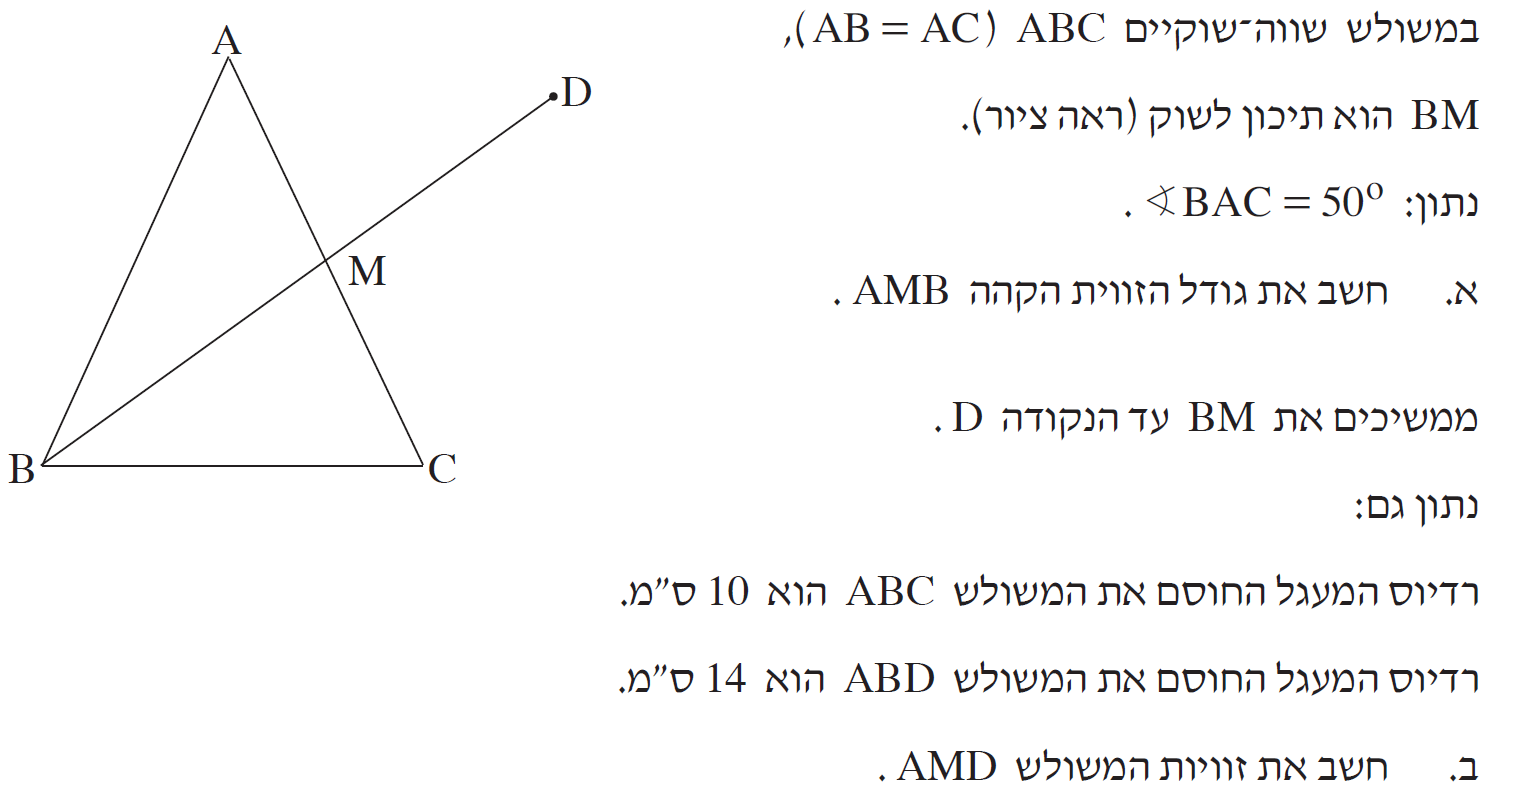
\includegraphics[width=.9\textwidth]{summer-2014a-5}
\end{center}



נסמן
$\alpha=\angle AMB$.
נתון 
$\angle BAC=50$
ובמשולש שווה-שוקיים
$\angle ABC=\angle ACB=(180-50)/2=65$.
נחשב
$\angle ABM=180-50-\alpha=130-\alpha$.


\begin{center}
\selectlanguage{english}
\begin{tikzpicture}[scale=.9]
\draw[thick] (0,0) coordinate (B) -- (5,0) coordinate (C);
\draw[thick] (B) -- node[left] {$a$} (2.5,6) coordinate (A);
\draw[thick,name path=ac] (A) -- (C);
\fill (B) node[below left] {$B$} node[above right,xshift=4pt] {$65$} circle(1.5pt);
\fill (A) node[above] {$A$} node[below,yshift=-16pt] {$50$} circle(1.5pt);
\fill (C) node[below right] {$C$} node[above left,xshift=-4pt] {$65$} circle(1.5pt);
\coordinate (M) at ($(A)!.5!(C)$);
\fill (M) node[below right,xshift=4pt,yshift=2pt] {$M$} node[left,yshift=2pt] {$\alpha$}  circle(1.5pt);
\draw[thick] (B) -- (M);
\path (A) -- node[right] {$a/2$} (M);
\path (M) -- node[right] {$a/2$} (C);
\node at ($(B)+(-25pt,25pt)$) {$130\!-\!\alpha$};
\draw[->] ($(B)+(0,25pt)$) -- +(18pt,0);
\end{tikzpicture}
\end{center}

\vspace{-3ex}


\textbf{סעיף א}


נחפש משולש שעליו אפשר להפעיל את חוק הסינוסים. נתון ש-%
$BM$
הוא תיכון ל-%
$AC$.
נסמן את 
$AB,AM$
עם הנעלם
$a$,
ונפעיל את משפט הסינוסים על
$\triangle ABM$.

\vspace{-3ex}


\erh{12pt}
\begin{equationarray*}{rcl}
\frac{a}{\sin\alpha}&=&\frac{a/2}{\sin(130-\alpha)}\\
\sin \alpha &=& 2\sin(130-\alpha)\\
&=&2\sin 130\cos \alpha - 2\sin\alpha \cos 130\\
&=&1.53\cos\alpha + 1.29\sin\alpha
\end{equationarray*}

\np

\erh{12pt}
\begin{equationarray*}{rcl}
\tan \alpha &=& -\frac{1.53}{0.29}\\
\alpha&=&-79.27^\circ = 100.73^\circ\approx 101^\circ\,.
\end{equationarray*}
בהמשך נעבוד עם קירובים למעלה שלמה.

\textbf{סעיף ב}

\begin{center}
\selectlanguage{english}
\begin{tikzpicture}[scale=.9]
\clip(-2,-1.1) rectangle +(11,7.6);
\draw[thick] (0,0) coordinate (B) -- (5,0) coordinate (C);
\draw[thick] (B) -- node[left] {$a$} (2.5,6) coordinate (A);
\draw[thick,name path=ac] (A) -- (C);
\fill (B) node[below left] {$B$} circle(1.5pt);
\fill (A) node[above] {$A$} circle(1.5pt);
\fill (C) node[below right] {$C$} node[above left,xshift=-4pt] {$65$}circle(1.5pt);
\coordinate (M) at ($(A)!.5!(C)$);
\fill (M) node[below right,xshift=4pt,yshift=2pt] {$M$} node[left,yshift=2pt] {$101$} node[above,xshift=3pt,yshift=7pt] {$79$}  circle(1.5pt);
\draw[thick] (B) -- ($(B)!1.8!(M)$) coordinate (D);
\fill (D) node[right] {$D$} node[below left,xshift=-12pt,yshift=2pt] {$\beta$} circle(1.5pt);
\path (A) -- (M);
\path (M) -- (C);
\tkzCircumCenter(A,B,C)\tkzGetPoint{C1}
\tkzDrawCircle[thick,dotted,name path=circle](C1,A)
\tkzCircumCenter(A,B,D)\tkzGetPoint{D1}
\tkzDrawCircle[thick,dotted,name path=circle](D1,A)
\draw[thick,dashed] (A) -- (D);
\end{tikzpicture}
\end{center}

$\angle AMB-101$
ולכן
$\angle AMD=$
לפי זוויות משלימות. נצטרך לחשב אחת מ-%
$\angle MAD,\angle ADM$,
והזווית השלישית תתקבל מסכום הזוויות במשולש. מהתרשים רואים שהצלע 
$AB$
מול הזווית
$\beta=\angle ADM$
היא באורך
$a$,
ו-%
$AB$
היא גם צלע מול
$\angle AMB=101$.
לפי חוק הסינוסים ב-%
$\angle ACB$, $\angle ADB$:

\vspace{-4ex}

\erh{10pt}
\begin{equationarray*}{rcl}
2R_{ABC}&=&\frac{a}{\sin 65}=2\cdot 10\\
a &=& 18.126\\
2R_{ABD}&=&\frac{a}{\sin \beta}=\frac{18.126}{\sin \beta}=2\cdot 14\\
\beta &=& 40.34\,.
\end{equationarray*}
הזוויות של
$\triangle AMD$
הן
$79^\circ, 40^\circ, 61^\circ$.


%%%%%%%%%%%%%%%%%%%%%%%%%%%%%%%%%%%%%%%%%%%%%%%%%%%%%%%%%%%%%%
\np

\section{חורף תשע"ד}

\begin{center}
\selectlanguage{english}
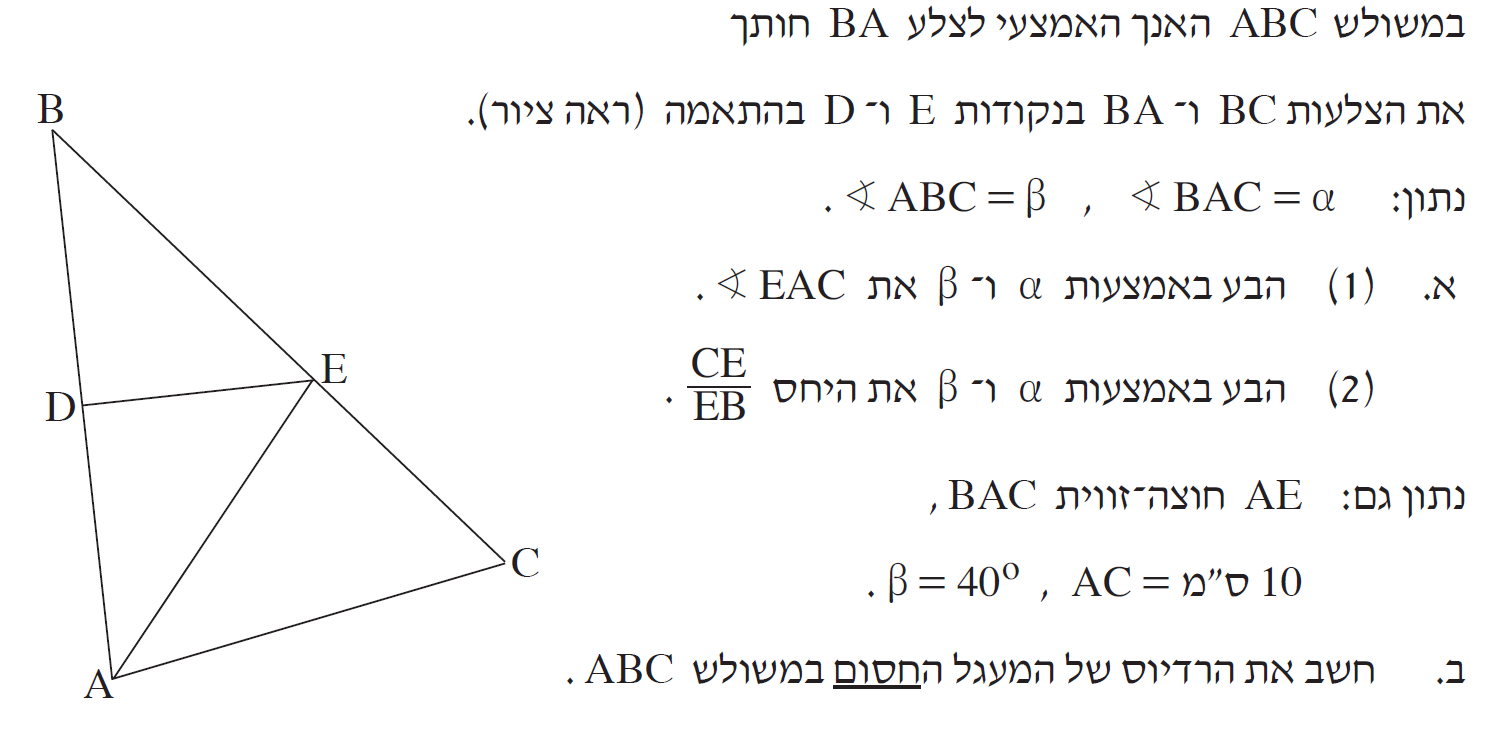
\includegraphics[width=.9\textwidth]{winter-2014-5}
\end{center}

\vspace{-2ex}

\textbf{סעיף א}

$(1)$
$DE$
הוא האנך האמצעי ל-%
$AB$,
ולכן
$\triangle AED\cong BED$
לפי צ.ז.צ. נסמן את שאר הזוויות לפי זוויות משלימות וסכום זוויות במשולש, כאשר קיצרנו
$\beta'=90\!-\!\beta$.
התשובה היא
$\angle EAC=\alpha\!-\!\beta$.

\vspace{-3ex}

\begin{center}
\selectlanguage{english}
\begin{tikzpicture}[scale=.85]
\draw[thick] (0,0) coordinate (A) -- (5,1) coordinate (C);
\draw[thick] (A) -- (100:8) coordinate (B);
\draw[thick,name path=bc] (B) -- (C);
\coordinate (D) at ($(A) ! .5 ! (B)$);
\fill (A) node[below left] {$A$} node[above right,xshift=10pt,yshift=14pt] {$\alpha$} node[above,xshift=4pt,yshift=20pt] {$\beta$} circle(1.5pt);
\fill (B) node[above] {$B$} node[below right,xshift=4pt,yshift=-16pt] {$\beta$} circle(1.5pt);
\fill (C) node[right] {$C$} node[above right,xshift=-4pt,yshift=6pt] {$180-(\alpha+\beta)$} circle(1.5pt);
\draw[->] ($(C)+(0pt,12pt)$) -- +(-14pt,-8pt);
\fill (D) node[left] {$D$} circle(1.5pt);
\path[name path=de] (D) -- +(10:4);
\path[name intersections={of=bc and de,by={E}}];
\fill (E) node[right] {$E$} node[above left,xshift=-8pt,yshift=-4pt] {$\beta'$} node[below left] {$\beta'$} node[below,xshift=4pt,yshift=-12pt] {$2\beta$}   circle(1.5pt);
\draw[thick] (D) -- (E);
\draw[thick,name path=ae] (A) -- (E);
\path (A) -- node[left] {$a$} (D);
\path (D) -- node[left] {$a$} (B);
\path (C) -- node[right] {$c$} (E);
\path (E) -- node[right,xshift=2pt] {$b$} (B);
\path (E) -- node[right] {$b$} (A);
\draw[rotate=10] (D) rectangle +(7pt,7pt);
\draw[very thick] ($(A)+(10:10mm)$) arc[start angle=25,end angle=101,radius=10mm];
\end{tikzpicture}
\end{center}

\vspace{-2ex}

$(2)$
נסמן 
$BE=b$,$EC=c$.
השאלה מבקשת את היחס
$\displaystyle\frac{c}{b}$.
מהתרשים נראה ש-%
$\angle BAC=\alpha=90$
ונוכל להשתמש במשפט תאלס, אבל אי אפשר להסתמך על התרשמות מהתרשים. הראנו ש-%
$\triangle AED\cong BED$,
כך ש-%
$AE=BE=b$,
ונוכל להשתמש בחוק הסינוסים ב-%
$\triangle AEC$:

\vspace{-6ex}

\erh{12pt}
\begin{equationarray*}{rcl}
\frac{c}{\sin (\alpha-\beta)}&=&\frac{b}{\sin(180-(\alpha+\beta))}\\
\frac{c}{b}&=&\frac{\sin (\alpha-\beta)}{\sin (\alpha+\beta)}\,.
\end{equationarray*}

\vspace{-2ex}

\np

\textbf{סעיף ב}

המשפט הרלוונטי הוא
$49$
"שלושת חוצי הזוויות של משולש נחתכים בנקודה אחת, שהיא מרכז המעגל החסום במשולש". נתון חוצה זווית 
$AE$
ב-%
$A$.
נבנה חוצה זווית שני. ננסה ב-%
$C$
כי ידוע
$AC=10$
ונוכל להשתמש בחוק הסינוסים ב-%
$\triangle ACF$,
כאשר 
$F$ 
היא נקודת החיתוך עם חוצה הזוויות 
$AE$,
ולכן היא המרכז של המעגל החסום.

נתון ש-%
$\beta=40$
וזה מאפשר לנו להשלים זוויות בתרשים:

\begin{center}
\selectlanguage{english}
\begin{tikzpicture}[scale=.85]
\draw[thick] (0,0) coordinate (A) -- (5,1) coordinate (C);
\draw[thick] (A) -- (100:8) coordinate (B);
\draw[thick,name path=bc] (B) -- (C);
\coordinate (D) at ($(A) ! .5 ! (B)$);
\fill (A) node[below left] {$A$} node[above right,xshift=10pt,yshift=10pt] {$40$} node[above,xshift=3pt,yshift=18pt] {$40$} circle(1.5pt);
\fill (B) node[above] {$B$} node[below right,xshift=3pt,yshift=-18pt] {$40$} circle(1.5pt);
\fill (C) node[right] {$C$} node[left,xshift=-14pt,yshift=2pt] {$30$} node[above left,xshift=-16pt,yshift=8pt] {$30$} circle(1.5pt);
\fill (D) node[left] {$D$} circle(1.5pt);
\path[name path=de] (D) -- +(10:4);
\path[name intersections={of=bc and de,by={E}}];
\fill (E) node[right] {$E$} node[above left,xshift=-8pt,yshift=-4pt] {$50$} node[below left,xshift=-3pt,yshift=-2pt] {$50$} node[below,xshift=4pt,yshift=-12pt] {$80$}   circle(1.5pt);
\draw[thick] (D) -- (E);
\draw[thick,name path=ae] (A) -- (E);
\path (A) -- node[left] {$a$} (D);
\path (D) -- node[left] {$a$} (B);
\path (C) -- node[right] {$c$} (E);
\path (E) -- node[right,xshift=2pt] {$b$} (B);
\path (E) -- node[right,xshift=4pt,yshift=10pt] {$b$} (A);
\path (A) -- node[below] {$10$} (C);
\draw[rotate=10] (D) rectangle +(7pt,7pt);
\path[name path=cf] (C) -- +(160:5);
\path[name intersections={of=ae and cf,by={F}}];
\fill (F) node[left] {$F$} node[below,xshift=8pt,yshift=-8pt] {$110$} circle(1.5pt);
\draw[thick] (C) -- node[above] {$x$} (F);
\end{tikzpicture}
\end{center}

\vspace{-3ex}

לפי חוק הסינוסים:

\vspace{-4ex}

\erh{14pt}
\begin{equationarray*}{rcl}
\frac{x}{\sin 40}&=&\frac{10}{\sin 110}\\
x &=& 6.84\,.
\end{equationarray*}
\textbf{לא לעצור כאן!}
השאלה מבקשת את הרדיוס של המעגל החסום ולא המרחק אל מרכז המעגל. 

נוריד אנך מ-%
$F$
ל-%
$AC$
ונחשב:
$r=x\sin 30 = 3.42$.
\begin{center}
\selectlanguage{english}
\begin{tikzpicture}[scale=.9]
\clip(-1.1,-.6) rectangle +(8.5,5.3);
\coordinate (A) at (0,0);
\draw[thick] (A) -- +(90:8) coordinate (B);
\path[name path=bc] (B) -- +(-50:10);
\path[name path=ac] (A) -- +(10:7);
\path[name intersections={of=ac and bc,by={C}}];
\draw[thick] (A) -- (C) -- (B);
\fill (B) node[above] {$B$};
\fill (A) node[below left] {$A$} node[above right,xshift=10pt,yshift=4pt] {$40$} circle(1.5pt);
\fill (C) node[right] {$C$} node[left,xshift=-14pt,yshift=2pt] {$30$} circle(1.5pt);
\path[name path=af] (A) -- +(50:5);
\path[name path=cf] (C) -- +(160:6);
\path[name intersections={of=af and cf,by={F}}];
\fill (F) node[above] {$F$} circle(1.5pt);
\draw[thick] (A) -- (F) -- node[above,near start] {$x$} (C);
\coordinate (G) at ($(A)!(F)!(C)$);
\draw[very thick,dashed]  (G) -- node[left] {$r$} (F);
\draw[rotate=10] (G) rectangle +(7pt,7pt);
\fill (G) circle(1.5pt);
\node[draw,very thick,dotted,circle through=(G)] at (F) {};
\end{tikzpicture}
\end{center}

\section{חורף תשע"ד )שאלה
$6$(}

\textbf{בבחינה זו היו שלוש שאלות בפרק השני.}

\begin{center}
\selectlanguage{english}
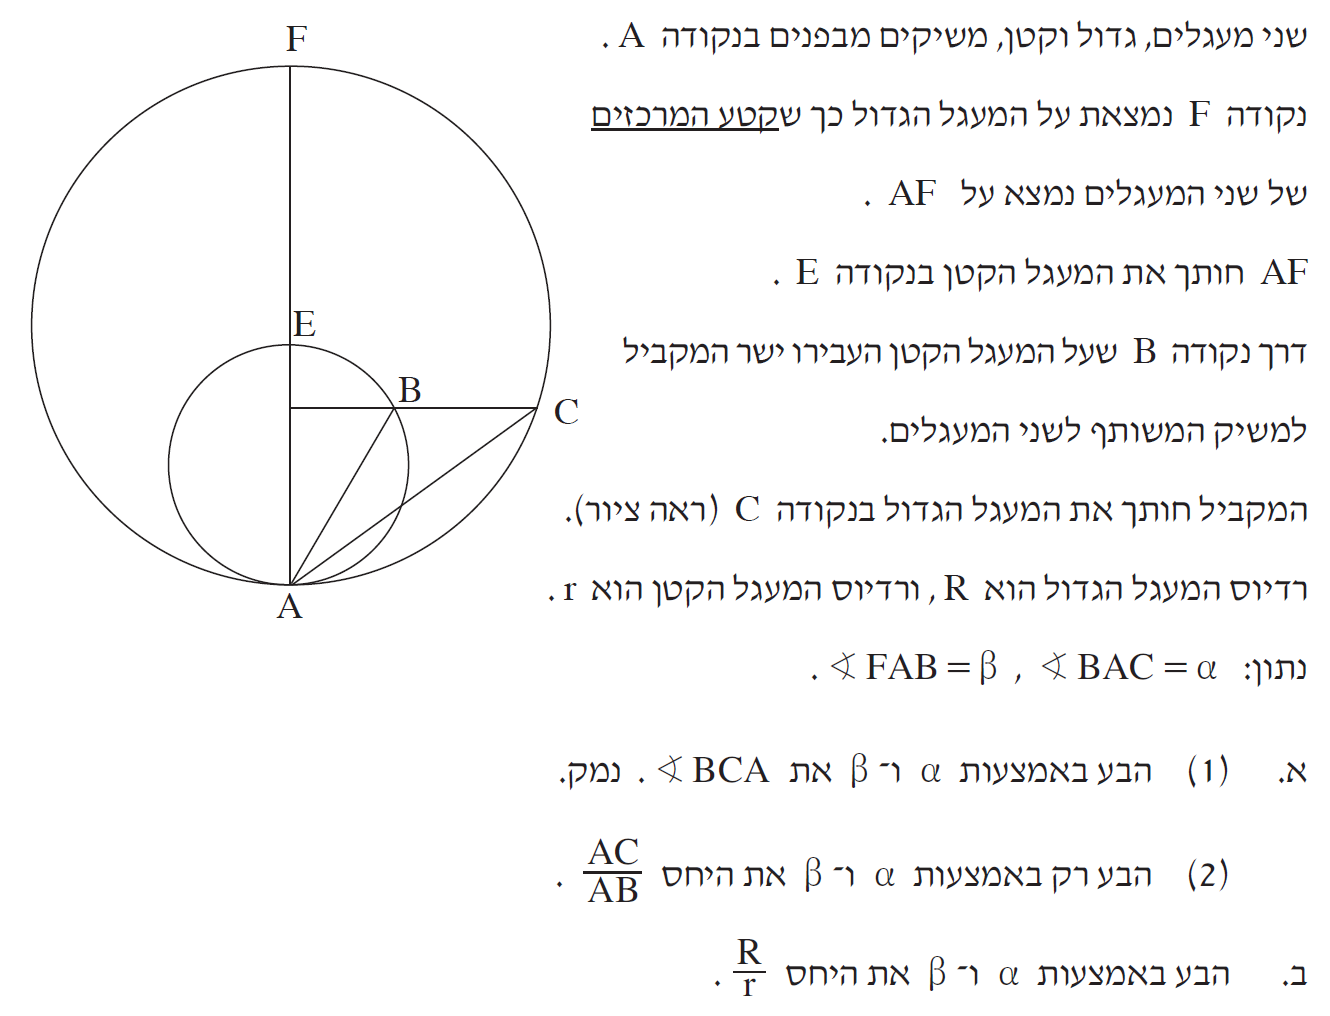
\includegraphics[width=.95\textwidth]{winter-2014-6}
\end{center}

\vspace{-2ex}

\begin{center}
\selectlanguage{english}
\begin{tikzpicture}[scale=.8]
\coordinate (O) at (0,0);
\coordinate (A) at (0,-4);
\coordinate (F) at (0,4);
\fill (A) circle(1.5pt) node[below] {$A$} node[above right,yshift=18pt,xshift=11pt] {$\alpha$} node[above,yshift=15pt,xshift=6pt] {$\beta$};
\fill (F) circle(1.5pt) node[above] {$F$};
\node[draw,thick,circle through=(A),name path=big-circle] (circle) at (O) {};
\node[draw,thick,circle through=(A),name path=small-circle] (circle) at (0,-2.1) {};
\draw[thick,name path=diameter] (A) -- (F);
\path[name intersections={of=diameter and small-circle,by={E}}];
\fill (E) circle(1.5pt) node[above left] {$E$};
\path[name path=ab] (A) -- +(65:5);
\path[name intersections={of=ab and small-circle,by={B}}];
\draw[thick] (A) -- (B);
\fill (B) circle(1.5pt) node[above right] {$B$};
\coordinate (D) at (A|-B);
\fill (D) circle(1.5pt) node[left] {$D$};
\path[name path=dc] (D) -- ($(D)!3!(B)$);
\path[name intersections={of=dc and big-circle,by={C}}];
\draw[thick] (D) -- (C);
\fill (C) circle(1.5pt) node[right] {$C$} node[below left,xshift=-12pt] {$\gamma$};
\draw[thick] (A) -- (C);
\draw[thick,rotate=-90] (D) rectangle +(8pt,8pt);
%\node at (1.8,1.5) {$\gamma = 90\!-\!(\alpha\!+\!\beta)$};
\draw[thick,dashed] (F) -- (C);
\draw[thick,dashed] (B) -- (E);
\draw[thick,rotate=130] (C) rectangle +(8pt,8pt);
\draw[thick,rotate=153] (B) rectangle +(8pt,8pt);
\end{tikzpicture}
\end{center}

\vspace{-4ex}

\textbf{סעיף א}

$(1)$
$\triangle DCA$ 
יישר זווית ולכן סכום הזזויות החדות שווה ל-%
$90$. $\angle BCA=\gamma=90-(\alpha+\beta)$.

\np

$(2)$
$AD$
הוא צלע של
$\triangle DCA$
וגם של
$\triangle DBA$.
נפעיל את חוק הסינוסים פעמיים:
\erh{12pt}
\begin{equationarray*}{rcl}
\frac{AB}{\sin 90}&=&\frac{AD}{\sin (90-\beta)}\\
AD&=&AB\cos \beta\\
\frac{AC}{\sin 90}&=&\frac{AD}{\sin \gamma}\\
AC&=&\frac{AB\cos\beta}{\sin(90-(\alpha+\beta))}\\
\frac{AC}{AB}&=&\frac{\cos\beta}{\cos(\alpha+\beta)}\,.
\end{equationarray*}
פתרון אחר מתקבל מהפעלת חוק הסינוסים פעם אחת על
$\triangle ABC$:
\erh{12pt}
\begin{equationarray*}{rcl}
\frac{AC}{\sin(180-\alpha-\gamma)}&=&\frac{AB}{\sin\gamma}\\
\frac{AC}{AB}&=&\frac{\sin(180-(\alpha+\gamma))}{\sin(90-(\alpha+\beta))}=\frac{\sin(\alpha+\gamma)}{\cos(\alpha+\beta)}\\
&=&\frac{\sin(\alpha+90-(\alpha+\beta))}{\cos(\alpha+\beta)}=\frac{\cos\beta}{\cos(\alpha+\beta)}
\end{equationarray*}


\textbf{סעיף ב}

לאחר שחישבנו יחס
$\frac{AC}{AB}$
נחפש קשר בין
$AB,AC$
לבין הרדיוסים. נחבר 
$B$
ל-%
$E$
ו-%
$C$
ל-%
$F$.
נקבל שני משולשים חסומים במעגלים וניתן להשתמש בנוסחה של חוק הסינוסים עם רדיוס:
\erh{14pt}
\begin{equationarray*}{rcl}
2R&=&\frac{AC}{\sin(90-(\alpha+\beta))}\\
2r&=&\frac{AB}{\sin(90-\beta)}\\
\frac{R}{r}&=&\frac{AC}{2\cos(\alpha+\beta)}\cdot \frac{2\cos\beta}{AB}=
=\frac{\cos^2\beta}{\cos^2(\alpha+\beta)}\
\end{equationarray*}
פתרון אחר: נתון ש-%
$FA$
הוא קוטר )"קטע המרכזים"( של המגעל הגדול, ולכן 
$EA$
הוא קוטר של המעגל הקטן. זווית הנשענת על קוטר
$\triangle ACF,\triangle ABE$
הן ישר-זווית, ולכן:
\erh{14pt}
\begin{equationarray*}{rcl}
\cos \beta &=& \frac{AB}{2r}\\
\cos (\alpha+\beta) &=& \frac{AC}{2R}\\
\frac{R}{r}&=&\frac{AC}{2\cos(\alpha+\beta)}\cdot \frac{2\cos\beta}{AB}=\frac{\cos^2\beta}{\cos^2(\alpha+\beta)}\,.
\end{equationarray*}

\np

\section*{המלצות: טריגונומטריה}

\addcontentsline{cot}{chapter}{המלצות: טריגונומטריה}


\begin{itemize}

\item
ראו נספח~%
\ref{a.unit-circle}
המסביר את החשיבות של מעגל היחידה בחישובים טריגונומטריים.

הנספח מציג איך לשחזר בקלות את הנוסחאות ל-%
$\sin 2\theta$, $\sin (180^\circ-\theta)$, $\sin (90^\circ-\theta)$,
ונוסאות דומות עבור קיסינוס.

\item
חשוב לצייר תרשימים 
\textbf{ברורים וגדולים},
עדיף עם סרגל ומחוגה. בתהליך הפתרון אנו מסמנים את המידע המצטבר על הזוויות והצלעות ויש לדאוג שיהיה מספיק מקום.

\item
כאשר לשאלה יש מספר סעיפים כדאי לצייר תרשימים נפרדים לכל סעיף תוך העלמת מידע לא רלוונטי לאותו סעיף.

\item
אני מעדיף לסמן זוויות עם אותיות יווניות כגון
$\alpha$,
ולא על ידי ציון שלושת הנקודות המגדירות אותה
$\angle ABC$,
כי קשה יותר לעקוב אחר הנקודות המגדירות את הזווית.

\item
השלימו זוויות ככל האפשר תוך שימוש בסכום הזוויות במשולש, ובזוויות משלימות. כדי להקל על החישובים אני משתמש בנעלמים נוספים כדי לקצר ביטויים, למשל,
$\gamma=180-(\alpha+\beta)$.

\item
שימו לב שאין עקביות בסימון 
$A,B,C,D$
של הקודקודים של משולש או מרובע.


\item 
בשאלות על טריגונומטריה בדרך כלל עדיף להשתמש בנוסחה לשטח משולש:
\[
S=\frac{1}{2}\cdot b \cdot c \cdot\sin \alpha\,,
\]
ולא בחישוב של מחצית מכפלת הבסיס והגובה.

\item
עבור מעגל חוסם במשולש, המשפט הרלוונטי הוא
$54$
"במשולש, שלושת האנכים האמצעיים נחתכים בנקודה אחת , שהיא מרכז המעגל החוסם את המשולש". ניתן בקלות למצוא את רדיוס המעגל מחוק הסינוסים:
\[
2R=\frac{a}{\sin\alpha}\,.
\]
\vspace{-4ex}
\item
עבור מעגל חסום במשולש, המשפט הרלוונטי הוא
$49$
"שלושת חוצי הזוויות של משולש נחתכים בנקודה אחת, שהיא מרכז המעגל החסום במשולש". אין נוסחה עבור רדיוס המעגל אבל אפשר למצוא אותו כאורך הגובה מהמרכז לאחת הצלעות.


\item 
טרפזים מאוד אהובים על ידי כותבי הבחינות. שננו משפטים
$56$
"ניתן לחסום מרובע במעגל אם ורק אם סכום זוג זוויות נגדיות שווה ל-%
$180$"
ו-%
$57$
"מרובע קמור חוסם מעגל אם ורק אם סכום שתי צלעות נגדיות שווה לסכום שתי הצלעות הנגדיות האחרות".

\item
שימו לב שהמרכז המעגל החוסם לא חופף את מרכז המעגל החסום, אלא במקרים מיוחדים כגון משולש שווה-צלעות וריבוע.


\item
לעתים קרובות התשובה לשאלה תהיה ערך ממשי לזווית או אורך. אני מעדיף להישאר עם נעלמים כל עוד הדבר אפשרי ורק בסוף להשתמש במחשבון כדי לחשב ערכים.


\end{itemize}

\npchap
